% answers.tex —— 2012 年·四川卷·理科 · 参考答案与详细解析片段
% 由 tools/generate_projects.py 依来源总账自 2012/2012_数学真题_四川理_试题.md + 2012/2012_数学真题_四川理_解析正文.md + 2012/2012_数学真题_四川理_答案要点.md 生成，勿手改（改源 MD 后重跑）

\begin{answer}
\gksolhead{1}{}

\textbf{题目}：

$(1+x)^7$ 的展开式中 $x^2$ 的系数是\mbox{（　　）}

（A）$42$；（B）$35$；（C）$28$；（D）$21$。

\Needspace{4\baselineskip}
\textbf{解析}

\Needspace{5\baselineskip}
二项展开式的通项为 $\mathrm T_{k+1}=\mathrm C_7^kx^k$，取 $k=2$ 得 $x^2$ 的系数
\nopagebreak[4]
\[\mathrm C_7^2=\frac{7\times6}{2}=21.\]
选 D。

\gkanswer{答案：D。}

\end{answer}
\begin{answer}
\gksolhead{2}{}

\textbf{题目}：

复数 $\dfrac{(1-\mathrm i)^2}{2\mathrm i}=$\mbox{（　　）}

（A）$1$；（B）$-1$；（C）$\mathrm i$；（D）$-\mathrm i$。

\Needspace{4\baselineskip}
\textbf{解析}

\Needspace{5\baselineskip}
先算分子：$(1-\mathrm i)^2=1-2\mathrm i+\mathrm i^2=-2\mathrm i$。故
\nopagebreak[4]
\[\frac{(1-\mathrm i)^2}{2\mathrm i}=\frac{-2\mathrm i}{2\mathrm i}=-1.\]
选 B。

\gkanswer{答案：B。}

\end{answer}
\begin{answer}
\gksolhead{3}{}

\textbf{题目}：

函数 $f(x)=\begin{cases}\dfrac{x^2-9}{x-3},&x<3,\\[4pt]\ln(x-2),&x\geqslant3,\end{cases}$ 在 $x=3$ 处的极限是\mbox{（　　）}

（A）不存在；（B）等于 $6$；（C）等于 $3$；（D）等于 $0$。

\Needspace{4\baselineskip}
\textbf{解析}

分别求左右极限。

\Needspace{5\baselineskip}
左极限（$x\to3^-$，此时 $x<3$，取 $f(x)=\dfrac{x^2-9}{x-3}$）：
\nopagebreak[4]
\[\lim_{x\to3^-}\frac{x^2-9}{x-3}=\lim_{x\to3^-}(x+3)=6.\]
\Needspace{5\baselineskip}
右极限（$x\to3^+$，此时 $x>3$，取 $f(x)=\ln(x-2)$）：
\nopagebreak[4]
\[\lim_{x\to3^+}\ln(x-2)=\ln1=0.\]
左右极限不相等（$6\neq0$），故 $f(x)$ 在 $x=3$ 处的极限不存在。选 A。

\gkanswer{答案：A。}

\end{answer}
\begin{answer}
\gksolhead{4}{}

\textbf{题目}：

如图，正方形 $ABCD$ 的边长为 $1$，延长 $BA$ 至 $E$，使 $AE=1$，连接 $EC$，$ED$，则 $\sin\angle CED=$\mbox{（　　）}
\nopagebreak[4]
\begin{center}%% ============================================================
% f2012_sichuan_sci_q04_square.tex
%% 2012 四川卷（理科）第 4 题 正方形 ABCD，延长 BA 至 E 使 AE=1
%% 来源 PDF：普通高考/2012/2012四川理.pdf 第 1 页（印面 771）第 1 栏
%% 坐标取自原页矢量层（bp），原点为图区左上角 (170.0,355.0)，y 向下。
%% ============================================================
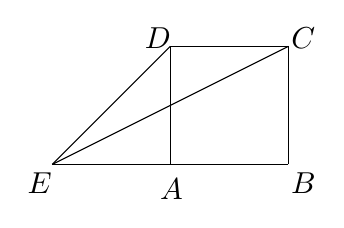
\begin{tikzpicture}[x=1bp,y=-1bp,
  every node/.style={inner sep=0,font=\fontsize{10.5pt}{12.6pt}\selectfont},
  line cap=butt, line join=miter]
  \draw[line width=0.398bp] (10.828,53.777) -- (95.836,53.777);
  \draw[line width=0.398bp] (95.836,11.273) -- (53.332,11.273);
  \draw[line width=0.398bp] (10.828,53.777) -- (95.836,11.273);
  \draw[line width=0.398bp] (95.836,53.777) -- (95.836,11.273);
  \draw[line width=0.398bp] (10.828,53.777) -- (53.332,11.273);
  \draw[line width=0.398bp] (53.332,53.777) -- (53.332,11.273);
  \node[anchor=base west] at (43.99,12.0) {$D$};
  \node[anchor=base west] at (96.74,12.0) {$C$};
  \node[anchor=base west] at (1.79,64.38) {$E$};
  \node[anchor=base west] at (49.48,66.43) {$A$};
  \node[anchor=base west] at (96.62,64.38) {$B$};
\end{tikzpicture}
\end{center}
\nopagebreak[4]
（A）$\dfrac{3\sqrt{10}}{10}$；（B）$\dfrac{\sqrt{10}}{10}$；（C）$\dfrac{\sqrt5}{10}$；（D）$\dfrac{\sqrt5}{15}$。

\Needspace{4\baselineskip}
\textbf{解析}

\Needspace{5\baselineskip}
取 $A(0,0)$，$B(1,0)$，$D(0,1)$，$C(1,1)$，由 $AE=1$ 且 $E$ 在 $BA$ 的延长线上得 $E(-1,0)$。则
\nopagebreak[4]
\[\overrightarrow{EC}=(2,1),\qquad \overrightarrow{ED}=(1,1).\]
\nopagebreak[4]
\[|\overrightarrow{EC}|=\sqrt5,\qquad |\overrightarrow{ED}|=\sqrt2,\qquad \overrightarrow{EC}\cdot\overrightarrow{ED}=2+1=3.\]
\Needspace{5\baselineskip}
故
\nopagebreak[4]
\[\cos\angle CED=\frac{3}{\sqrt5\cdot\sqrt2}=\frac{3}{\sqrt{10}},\]
\nopagebreak[4]
\[\sin\angle CED=\sqrt{1-\frac9{10}}=\frac{\sqrt{10}}{10}.\]
选 B。

\gkanswer{答案：B。}

\end{answer}
\begin{answer}
\gksolhead{5}{}

\textbf{题目}：

函数 $y=a^x-\dfrac1a$（$a>0$，$a\neq1$）的图象可能是\mbox{（　　）}
\nopagebreak[4]
\begin{center}%% ============================================================
% f2012_sichuan_sci_q05_graphs.tex
%% 2012 四川卷（理科）第 5 题 函数 y=a^x-1/a 的四个选项图象
%% 来源 PDF：普通高考/2012/2012四川理.pdf 第 1 页（印面 771）第 1 栏
%% 坐标取自原页矢量层（bp），原点为图区左上角 (60.0,485.0)，y 向下；
%% 曲线为原页折线路径逐点复刻（原页为示意画法，未按解析函数重拟合）。
%% 按原页刻度换算：四个子图 x 轴单位长约 17.0bp、y 轴单位长约 17.0bp。
%% ============================================================
\begin{tikzpicture}[x=1bp,y=-1bp,
  every node/.style={inner sep=0,font=\fontsize{10.5pt}{12.6pt}\selectfont},
  line cap=butt, line join=miter]
  \draw[line width=0.398bp] (95.141,76.543) -- (95.141,74.84);
  \draw[line width=0.398bp] (78.137,59.539) -- (79.84,59.539);
  \draw[line width=0.398bp] (27.133,76.543) -- (125.559,76.543);
  \fill[black] (129.145,76.543) .. controls (128.082,76.344) and (126.355,75.746) .. (125.16,75.047) -- (125.16,78.035) .. controls (126.355,77.34) and (128.082,76.742) .. (129.145,76.543);
  \draw[line width=0.398bp] (78.137,115.645) -- (78.137,12.121);
  \fill[black] (78.137,8.535) .. controls (77.938,9.598) and (77.34,11.324) .. (76.645,12.52) -- (79.633,12.52) .. controls (78.934,11.324) and (78.336,9.598) .. (78.137,8.535);
  \draw[line width=0.797bp] (35.633,73.535) -- (35.879,73.508) -- (36.121,73.477) -- (36.367,73.445) -- (36.609,73.414) -- (36.855,73.383) -- (37.102,73.348) -- (37.344,73.32) -- (37.59,73.289) -- (37.832,73.254) -- (38.078,73.219) -- (38.32,73.187) -- (38.566,73.156) -- (38.809,73.121) -- (39.301,73.051) -- (39.543,73.016) -- (39.789,72.98) -- (40.031,72.945) -- (40.277,72.91) -- (40.52,72.871) -- (40.766,72.836) -- (41.008,72.797) -- (41.254,72.762) -- (41.496,72.723) -- (41.988,72.645) -- (42.23,72.609) -- (42.477,72.566) -- (42.719,72.527) -- (42.965,72.488) -- (43.211,72.445) -- (43.453,72.406) -- (43.699,72.367) -- (43.941,72.324) -- (44.187,72.281) -- (44.43,72.238) -- (44.676,72.195) -- (44.918,72.152) -- (45.164,72.109) -- (45.41,72.062) -- (45.652,72.02) -- (45.898,71.973) -- (46.141,71.93) -- (46.387,71.883) -- (46.629,71.836) -- (46.875,71.785) -- (47.117,71.738) -- (47.609,71.645) -- (47.852,71.594) -- (48.098,71.547) -- (48.34,71.496) -- (48.586,71.441) -- (48.832,71.391) -- (49.316,71.289) -- (49.562,71.238) -- (49.809,71.184) -- (50.051,71.129) -- (50.297,71.078) -- (50.539,71.02) -- (51.031,70.91) -- (51.273,70.852) -- (51.52,70.797) -- (51.762,70.738) -- (52.008,70.68) -- (52.25,70.621) -- (52.496,70.563) -- (52.738,70.504) -- (52.984,70.445) -- (53.23,70.383) -- (53.473,70.32) -- (53.719,70.258) -- (53.961,70.195) -- (54.207,70.129) -- (54.449,70.066) -- (54.695,70.004) -- (54.937,69.938) -- (55.43,69.805) -- (55.672,69.738) -- (55.918,69.668) -- (56.16,69.602) -- (56.406,69.531) -- (56.648,69.461) -- (56.895,69.391) -- (57.141,69.316) -- (57.383,69.246) -- (57.629,69.172) -- (57.871,69.098) -- (58.117,69.023) -- (58.359,68.949) -- (58.605,68.871) -- (58.848,68.797) -- (59.34,68.641) -- (59.582,68.563) -- (59.828,68.48) -- (60.07,68.398) -- (60.316,68.32) -- (60.559,68.238) -- (60.805,68.152) -- (61.047,68.07) -- (61.539,67.898) -- (61.781,67.813) -- (62.027,67.723) -- (62.27,67.637) -- (62.762,67.457) -- (63.004,67.367) -- (63.246,67.273) -- (63.492,67.184) -- (63.738,67.086) -- (63.98,66.992) -- (64.227,66.898) -- (64.469,66.801) -- (64.961,66.605) -- (65.203,66.504) -- (65.449,66.406) -- (65.691,66.305) -- (65.937,66.199) -- (66.18,66.098) -- (66.426,65.992) -- (66.668,65.887) -- (66.914,65.781) -- (67.16,65.672) -- (67.402,65.563) -- (67.648,65.453) -- (67.891,65.34) -- (68.137,65.23) -- (68.379,65.117) -- (68.625,65.004) -- (68.867,64.887) -- (69.359,64.652) -- (69.602,64.535) -- (69.848,64.414) -- (70.09,64.293) -- (70.336,64.172) -- (70.578,64.047) -- (70.824,63.922) -- (71.07,63.793) -- (71.312,63.668) -- (71.559,63.539) -- (71.801,63.41) -- (72.047,63.273) -- (72.289,63.145) -- (72.535,63.008) -- (72.777,62.875) -- (73.023,62.738) -- (73.27,62.598) -- (73.512,62.461) -- (73.758,62.32) -- (74,62.176) -- (74.246,62.031) -- (74.488,61.887) -- (74.734,61.738) -- (74.977,61.594) -- (75.223,61.441) -- (75.469,61.293) -- (75.711,61.137) -- (75.957,60.984) -- (76.199,60.828) -- (76.445,60.672) -- (76.687,60.512) -- (76.934,60.352) -- (77.176,60.188) -- (77.422,60.027) -- (77.668,59.859) -- (77.91,59.691) -- (78.156,59.527) -- (78.398,59.359) -- (78.645,59.188) -- (78.891,59.012) -- (79.133,58.836) -- (79.379,58.66) -- (79.621,58.48) -- (79.867,58.301) -- (80.109,58.117) -- (80.355,57.934) -- (80.598,57.746) -- (80.844,57.559) -- (81.09,57.367) -- (81.332,57.176) -- (81.578,56.984) -- (81.82,56.785) -- (82.066,56.59) -- (82.309,56.391) -- (82.555,56.188) -- (82.797,55.984) -- (83.289,55.57) -- (83.531,55.359) -- (83.777,55.148) -- (84.02,54.934) -- (84.266,54.715) -- (84.512,54.5) -- (84.996,54.055) -- (85.488,53.602) -- (85.73,53.371) -- (85.977,53.141) -- (86.219,52.906) -- (86.465,52.672) -- (86.707,52.43) -- (86.953,52.191) -- (87.199,51.945) -- (87.441,51.699) -- (87.687,51.449) -- (87.93,51.199) -- (88.176,50.945) -- (88.418,50.691) -- (88.664,50.43) -- (88.906,50.168) -- (89.152,49.906) -- (89.398,49.637) -- (89.641,49.371) -- (89.887,49.098) -- (90.129,48.824) -- (90.375,48.547) -- (90.617,48.266) -- (90.863,47.98) -- (91.105,47.695) -- (91.598,47.117) -- (91.84,46.82) -- (92.086,46.523) -- (92.328,46.223) -- (92.82,45.613) -- (93.062,45.305) -- (93.309,44.988) -- (93.551,44.676) -- (93.797,44.355) -- (94.039,44.035) -- (94.285,43.707) -- (94.527,43.379) -- (94.773,43.047) -- (95.02,42.711) -- (95.262,42.375) -- (95.508,42.031) -- (95.75,41.684) -- (95.996,41.336) -- (96.238,40.984) -- (96.484,40.629) -- (96.727,40.27) -- (96.973,39.906) -- (97.219,39.539) -- (97.461,39.168) -- (97.707,38.793) -- (97.949,38.414) -- (98.195,38.035) -- (98.441,37.648) -- (98.926,36.867) -- (99.172,36.469) -- (99.418,36.066) -- (99.66,35.664) -- (99.906,35.254) -- (100.148,34.84) -- (100.395,34.422) -- (100.641,34) -- (100.883,33.574) -- (101.129,33.145) -- (101.371,32.711) -- (101.617,32.27) -- (101.859,31.828) -- (102.105,31.379) -- (102.348,30.93) -- (102.594,30.473) -- (102.836,30.012) -- (103.328,29.074) -- (103.57,28.598) -- (103.816,28.117) -- (104.059,27.633) -- (104.305,27.145) -- (104.547,26.648) -- (104.793,26.148) -- (105.035,25.645) -- (105.281,25.137) -- (105.527,24.621) -- (105.77,24.102) -- (106.016,23.578) -- (106.258,23.047) -- (106.504,22.512) -- (106.75,21.969) -- (106.992,21.422) -- (107.238,20.871) -- (107.48,20.316) -- (107.727,19.75) -- (107.969,19.184) -- (108.215,18.609) -- (108.457,18.027) -- (108.703,17.441);
  \draw[line width=0.398bp] (264.715,76.543) -- (264.715,74.84);
  \draw[line width=0.398bp] (247.711,59.539) -- (249.41,59.539);
  \draw[line width=0.398bp] (196.707,76.543) -- (295.133,76.543);
  \fill[black] (298.719,76.543) .. controls (297.656,76.344) and (295.93,75.746) .. (294.734,75.047) -- (294.734,78.035) .. controls (295.93,77.34) and (297.656,76.742) .. (298.719,76.543);
  \draw[line width=0.398bp] (247.711,115.645) -- (247.711,12.121);
  \fill[black] (247.711,8.535) .. controls (247.512,9.598) and (246.914,11.324) .. (246.219,12.52) -- (249.207,12.52) .. controls (248.508,11.324) and (247.91,9.598) .. (247.711,8.535);
  \draw[line width=0.797bp] (205.207,99.039) -- (205.465,99.008) -- (205.719,98.977) -- (205.977,98.941) -- (206.484,98.879) -- (206.742,98.844) -- (206.996,98.809) -- (207.254,98.777) -- (207.508,98.742) -- (207.766,98.707) -- (208.02,98.672) -- (208.277,98.637) -- (208.531,98.602) -- (208.789,98.566) -- (209.043,98.527) -- (209.301,98.492) -- (209.555,98.457) -- (209.812,98.418) -- (210.066,98.379) -- (210.324,98.34) -- (210.578,98.301) -- (210.836,98.262) -- (211.09,98.223) -- (211.348,98.184) -- (211.602,98.145) -- (211.859,98.102) -- (212.113,98.059) -- (212.371,98.02) -- (212.625,97.977) -- (212.883,97.934) -- (213.137,97.891) -- (213.395,97.848) -- (213.648,97.805) -- (213.902,97.758) -- (214.16,97.715) -- (214.414,97.668) -- (214.672,97.625) -- (214.926,97.574) -- (215.184,97.531) -- (215.437,97.48) -- (215.695,97.434) -- (215.949,97.387) -- (216.207,97.336) -- (216.461,97.289) -- (216.719,97.238) -- (216.973,97.188) -- (217.23,97.137) -- (217.484,97.086) -- (217.742,97.031) -- (217.996,96.98) -- (218.254,96.93) -- (218.508,96.871) -- (218.766,96.82) -- (219.02,96.766) -- (219.277,96.711) -- (219.531,96.652) -- (219.789,96.598) -- (220.043,96.539) -- (220.301,96.48) -- (220.555,96.426) -- (220.809,96.363) -- (221.066,96.305) -- (221.32,96.246) -- (221.578,96.184) -- (221.832,96.125) -- (222.09,96.059) -- (222.344,96) -- (222.602,95.934) -- (222.859,95.871) -- (223.113,95.809) -- (223.367,95.742) -- (223.625,95.676) -- (223.879,95.609) -- (224.137,95.539) -- (224.391,95.473) -- (224.648,95.406) -- (224.902,95.336) -- (225.16,95.262) -- (225.414,95.195) -- (225.672,95.121) -- (225.926,95.047) -- (226.184,94.977) -- (226.437,94.902) -- (226.695,94.824) -- (226.949,94.75) -- (227.207,94.672) -- (227.461,94.598) -- (227.719,94.52) -- (227.973,94.441) -- (228.227,94.359) -- (228.484,94.277) -- (228.742,94.199) -- (228.996,94.113) -- (229.254,94.031) -- (229.508,93.949) -- (229.766,93.863) -- (230.273,93.691) -- (230.531,93.602) -- (230.785,93.516) -- (231.043,93.426) -- (231.297,93.336) -- (231.555,93.246) -- (231.809,93.148) -- (232.066,93.059) -- (232.32,92.965) -- (232.578,92.867) -- (232.832,92.773) -- (233.09,92.676) -- (233.344,92.578) -- (233.602,92.477) -- (233.855,92.379) -- (234.113,92.277) -- (234.367,92.176) -- (234.625,92.07) -- (234.879,91.965) -- (235.137,91.859) -- (235.391,91.754) -- (235.648,91.645) -- (235.902,91.535) -- (236.16,91.426) -- (236.414,91.316) -- (236.672,91.203) -- (236.926,91.09) -- (237.184,90.973) -- (237.437,90.859) -- (237.691,90.742) -- (237.949,90.621) -- (238.203,90.504) -- (238.461,90.383) -- (238.715,90.258) -- (238.973,90.137) -- (239.227,90.012) -- (239.484,89.887) -- (239.738,89.758) -- (239.996,89.629) -- (240.25,89.5) -- (240.508,89.367) -- (240.762,89.234) -- (241.02,89.102) -- (241.273,88.965) -- (241.531,88.828) -- (241.785,88.688) -- (242.043,88.551) -- (242.297,88.406) -- (242.555,88.266) -- (242.809,88.121) -- (243.066,87.973) -- (243.32,87.828) -- (243.578,87.68) -- (243.832,87.527) -- (244.09,87.375) -- (244.344,87.219) -- (244.598,87.066) -- (244.855,86.906) -- (245.109,86.75) -- (245.367,86.59) -- (245.621,86.426) -- (245.879,86.262) -- (246.133,86.098) -- (246.391,85.934) -- (246.648,85.762) -- (247.156,85.418) -- (247.414,85.246) -- (247.668,85.07) -- (247.926,84.895) -- (248.18,84.715) -- (248.437,84.535) -- (248.691,84.348) -- (248.949,84.164) -- (249.203,83.977) -- (249.461,83.789) -- (249.715,83.598) -- (249.973,83.402) -- (250.227,83.207) -- (250.484,83.012) -- (250.738,82.809) -- (250.996,82.609) -- (251.25,82.406) -- (251.504,82.199) -- (251.762,81.992) -- (252.016,81.781) -- (252.273,81.57) -- (252.527,81.355) -- (253.043,80.918) -- (253.297,80.695) -- (253.555,80.473) -- (254.062,80.02) -- (254.32,79.789) -- (254.574,79.555) -- (254.832,79.32) -- (255.086,79.082) -- (255.344,78.84) -- (255.598,78.598) -- (255.855,78.352) -- (256.109,78.102) -- (256.367,77.852) -- (256.879,77.34) -- (257.133,77.082) -- (257.391,76.82) -- (257.645,76.555) -- (257.902,76.289) -- (258.156,76.02) -- (258.414,75.746) -- (258.668,75.473) -- (258.926,75.191) -- (259.18,74.91) -- (259.437,74.629) -- (259.691,74.34) -- (259.949,74.051) -- (260.203,73.754) -- (260.461,73.461) -- (260.715,73.16) -- (260.969,72.855) -- (261.227,72.551) -- (261.48,72.242) -- (261.738,71.93) -- (261.992,71.613) -- (262.25,71.293) -- (262.504,70.973) -- (262.762,70.648) -- (263.016,70.316) -- (263.273,69.984) -- (263.527,69.648) -- (263.785,69.309) -- (264.039,68.965) -- (264.297,68.621) -- (264.551,68.27) -- (264.809,67.914) -- (265.062,67.559) -- (265.32,67.195) -- (265.574,66.832) -- (265.832,66.461) -- (266.086,66.09) -- (266.344,65.711) -- (266.598,65.332) -- (266.855,64.945) -- (267.109,64.559) -- (267.367,64.164) -- (267.621,63.766) -- (267.879,63.367) -- (268.133,62.961) -- (268.387,62.551) -- (268.645,62.137) -- (268.898,61.719) -- (269.156,61.297) -- (269.41,60.867) -- (269.668,60.438) -- (269.922,60) -- (270.18,59.563) -- (270.434,59.113) -- (270.691,58.668) -- (270.945,58.211) -- (271.203,57.75) -- (271.457,57.285) -- (271.715,56.816) -- (271.969,56.344) -- (272.227,55.863) -- (272.48,55.379) -- (272.738,54.891) -- (272.992,54.398) -- (273.25,53.898) -- (273.504,53.395) -- (273.762,52.883) -- (274.016,52.367) -- (274.273,51.848) -- (274.527,51.32) -- (274.785,50.789) -- (275.039,50.254) -- (275.293,49.707) -- (275.551,49.16) -- (275.805,48.605) -- (276.062,48.047) -- (276.316,47.48) -- (276.832,46.332) -- (277.086,45.746) -- (277.344,45.156) -- (277.598,44.559) -- (277.852,43.957) -- (278.109,43.348) -- (278.363,42.734) -- (278.621,42.113) -- (278.875,41.484) -- (279.133,40.848) -- (279.387,40.207) -- (279.645,39.559) -- (279.898,38.906) -- (280.156,38.242) -- (280.41,37.574) -- (280.668,36.898) -- (280.922,36.215) -- (281.18,35.523) -- (281.434,34.828) -- (281.691,34.125);
  \draw[line width=0.398bp] (94.844,200.277) -- (94.844,198.578);
  \draw[line width=0.398bp] (77.844,183.273) -- (79.543,183.273);
  \draw[line width=0.398bp] (26.84,200.277) -- (125.266,200.277);
  \fill[black] (128.848,200.277) .. controls (127.785,200.078) and (126.059,199.48) .. (124.867,198.785) -- (124.867,201.77) .. controls (126.059,201.074) and (127.785,200.477) .. (128.848,200.277);
  \draw[line width=0.398bp] (77.844,239.383) -- (77.844,135.855);
  \fill[black] (77.844,132.27) .. controls (77.645,133.332) and (77.047,135.059) .. (76.352,136.254) -- (79.336,136.254) .. controls (78.641,135.059) and (78.043,133.332) .. (77.844,132.27);
  \draw[line width=0.797bp] (43.84,140.77) -- (44.098,141.492) -- (44.352,142.191) -- (44.609,142.883) -- (44.863,143.566) -- (45.117,144.238) -- (45.375,144.91) -- (45.629,145.574) -- (45.887,146.227) -- (46.141,146.879) -- (46.398,147.52) -- (46.652,148.156) -- (46.91,148.781) -- (47.164,149.406) -- (47.422,150.02) -- (47.676,150.633) -- (47.934,151.234) -- (48.187,151.832) -- (48.445,152.422) -- (48.699,153.008) -- (48.957,153.586) -- (49.211,154.156) -- (49.469,154.723) -- (49.723,155.285) -- (49.98,155.84) -- (50.234,156.387) -- (50.492,156.93) -- (50.746,157.469) -- (51.004,158) -- (51.258,158.527) -- (51.516,159.051) -- (51.77,159.566) -- (52.027,160.078) -- (52.281,160.582) -- (52.535,161.082) -- (52.793,161.578) -- (53.047,162.066) -- (53.305,162.551) -- (53.562,163.031) -- (53.816,163.504) -- (54.074,163.977) -- (54.582,164.898) -- (54.84,165.355) -- (55.094,165.805) -- (55.352,166.25) -- (55.605,166.691) -- (55.863,167.129) -- (56.117,167.559) -- (56.375,167.988) -- (56.629,168.41) -- (56.887,168.828) -- (57.141,169.242) -- (57.398,169.652) -- (57.652,170.059) -- (57.91,170.461) -- (58.164,170.859) -- (58.422,171.25) -- (58.676,171.641) -- (58.934,172.027) -- (59.441,172.785) -- (59.957,173.527) -- (60.211,173.895) -- (60.469,174.254) -- (60.723,174.613) -- (60.98,174.969) -- (61.234,175.316) -- (61.492,175.664) -- (61.746,176.008) -- (62,176.348) -- (62.258,176.684) -- (62.512,177.02) -- (62.77,177.348) -- (63.023,177.672) -- (63.281,177.996) -- (63.535,178.316) -- (63.793,178.633) -- (64.047,178.945) -- (64.305,179.254) -- (64.559,179.559) -- (64.816,179.863) -- (65.07,180.164) -- (65.328,180.461) -- (65.582,180.754) -- (65.84,181.043) -- (66.094,181.332) -- (66.352,181.617) -- (66.605,181.898) -- (66.863,182.176) -- (67.117,182.453) -- (67.375,182.727) -- (67.629,182.996) -- (67.887,183.262) -- (68.141,183.527) -- (68.398,183.789) -- (68.652,184.051) -- (68.906,184.305) -- (69.164,184.559) -- (69.418,184.812) -- (69.676,185.059) -- (69.93,185.305) -- (70.187,185.551) -- (70.441,185.789) -- (70.699,186.027) -- (70.953,186.266) -- (71.211,186.5) -- (71.465,186.73) -- (71.723,186.957) -- (71.977,187.184) -- (72.234,187.406) -- (72.488,187.629) -- (72.746,187.848) -- (73,188.066) -- (73.258,188.281) -- (73.512,188.492) -- (73.77,188.703) -- (74.023,188.914) -- (74.281,189.117) -- (74.535,189.324) -- (74.793,189.523) -- (75.047,189.723) -- (75.305,189.922) -- (75.559,190.117) -- (75.816,190.309) -- (76.324,190.691) -- (76.582,190.879) -- (76.836,191.066) -- (77.094,191.25) -- (77.348,191.43) -- (77.605,191.609) -- (77.863,191.785) -- (78.371,192.137) -- (78.629,192.309) -- (78.883,192.477) -- (79.141,192.648) -- (79.395,192.816) -- (79.652,192.98) -- (79.906,193.145) -- (80.164,193.305) -- (80.418,193.469) -- (80.676,193.625) -- (80.93,193.781) -- (81.187,193.937) -- (81.441,194.09) -- (81.699,194.246) -- (81.953,194.395) -- (82.211,194.543) -- (82.465,194.691) -- (82.723,194.84) -- (82.977,194.984) -- (83.23,195.125) -- (83.488,195.27) -- (83.746,195.406) -- (84,195.547) -- (84.258,195.684) -- (84.512,195.82) -- (84.77,195.953) -- (85.277,196.219) -- (85.535,196.352) -- (85.789,196.477) -- (86.047,196.605) -- (86.301,196.734) -- (86.559,196.859) -- (86.812,196.98) -- (87.07,197.102) -- (87.324,197.223) -- (87.582,197.344) -- (87.836,197.461) -- (88.094,197.582) -- (88.348,197.695) -- (88.605,197.812) -- (88.859,197.926) -- (89.117,198.035) -- (89.371,198.148) -- (89.629,198.258) -- (89.883,198.367) -- (90.141,198.477) -- (90.395,198.582) -- (90.652,198.687) -- (90.906,198.793) -- (91.164,198.898) -- (91.418,199) -- (91.676,199.102) -- (91.93,199.203) -- (92.187,199.301) -- (92.695,199.496) -- (92.953,199.594) -- (93.207,199.687) -- (93.465,199.781) -- (93.719,199.875) -- (93.977,199.969) -- (94.23,200.059) -- (94.488,200.148) -- (94.742,200.238) -- (95,200.328) -- (95.254,200.418) -- (95.512,200.504) -- (95.766,200.59) -- (96.023,200.672) -- (96.277,200.758) -- (96.535,200.84) -- (96.789,200.922) -- (97.047,201.004) -- (97.301,201.086) -- (97.559,201.164) -- (97.812,201.246) -- (98.07,201.324) -- (98.324,201.398) -- (98.582,201.477) -- (98.836,201.551) -- (99.094,201.625) -- (99.602,201.773) -- (99.859,201.848) -- (100.113,201.918) -- (100.371,201.988) -- (100.625,202.059) -- (100.883,202.129) -- (101.137,202.199) -- (101.395,202.266) -- (101.652,202.336) -- (101.906,202.398) -- (102.16,202.469) -- (102.418,202.535) -- (102.672,202.598) -- (102.93,202.664) -- (103.184,202.727) -- (103.441,202.789) -- (103.695,202.852) -- (103.953,202.91) -- (104.207,202.973) -- (104.465,203.031) -- (104.719,203.094) -- (104.977,203.152) -- (105.23,203.211) -- (105.488,203.27) -- (105.742,203.324) -- (106,203.383) -- (106.254,203.437) -- (106.512,203.492) -- (107.02,203.602) -- (107.277,203.656) -- (107.531,203.707) -- (107.789,203.762) -- (108.047,203.812) -- (108.301,203.863) -- (108.559,203.914) -- (109.066,204.016) -- (109.324,204.066) -- (109.578,204.113) -- (109.836,204.164) -- (110.09,204.211) -- (110.348,204.258) -- (110.602,204.305) -- (110.859,204.352) -- (111.113,204.398) -- (111.371,204.445) -- (111.625,204.488) -- (111.883,204.531) -- (112.137,204.574) -- (112.395,204.621) -- (112.648,204.664) -- (112.906,204.707) -- (113.16,204.746) -- (113.418,204.789) -- (113.672,204.832) -- (113.93,204.871) -- (114.184,204.914) -- (114.441,204.953) -- (114.695,204.992) -- (114.953,205.031) -- (115.207,205.07) -- (115.465,205.109) -- (115.719,205.148) -- (115.977,205.184) -- (116.23,205.223) -- (116.484,205.258) -- (116.742,205.297) -- (116.996,205.332) -- (117.254,205.367) -- (117.508,205.402) -- (117.766,205.437) -- (118.02,205.473) -- (118.277,205.508) -- (118.531,205.539) -- (118.789,205.574) -- (119.043,205.609) -- (119.301,205.641) -- (119.555,205.672) -- (119.812,205.707) -- (120.066,205.738) -- (120.324,205.77);
  \draw[line width=0.398bp] (265.301,200.277) -- (265.301,198.578);
  \draw[line width=0.398bp] (248.301,183.273) -- (250,183.273);
  \draw[line width=0.398bp] (197.293,200.277) -- (295.719,200.277);
  \fill[black] (299.305,200.277) .. controls (298.242,200.078) and (296.516,199.48) .. (295.32,198.785) -- (295.32,201.77) .. controls (296.516,201.074) and (298.242,200.477) .. (299.305,200.277);
  \draw[line width=0.398bp] (248.301,239.383) -- (248.301,135.855);
  \fill[black] (248.301,132.27) .. controls (248.102,133.332) and (247.504,135.059) .. (246.805,136.254) -- (249.793,136.254) .. controls (249.098,135.059) and (248.5,133.332) .. (248.301,132.27);
  \draw[line width=0.797bp] (214.297,171.375) -- (214.551,172.094) -- (214.809,172.793) -- (215.063,173.484) -- (215.32,174.168) -- (215.574,174.844) -- (215.832,175.516) -- (216.086,176.176) -- (216.344,176.832) -- (216.598,177.48) -- (216.855,178.121) -- (217.109,178.758) -- (217.367,179.387) -- (217.621,180.008) -- (217.875,180.625) -- (218.133,181.234) -- (218.387,181.836) -- (218.645,182.434) -- (218.898,183.027) -- (219.156,183.609) -- (219.41,184.187) -- (219.668,184.762) -- (219.922,185.328) -- (220.18,185.887) -- (220.434,186.441) -- (220.691,186.992) -- (220.945,187.535) -- (221.203,188.074) -- (221.457,188.605) -- (221.715,189.133) -- (221.969,189.652) -- (222.227,190.168) -- (222.48,190.68) -- (222.738,191.184) -- (222.992,191.684) -- (223.25,192.18) -- (223.504,192.668) -- (223.762,193.152) -- (224.016,193.633) -- (224.273,194.105) -- (224.527,194.578) -- (224.785,195.043) -- (225.293,195.957) -- (225.551,196.406) -- (225.805,196.852) -- (226.062,197.297) -- (226.316,197.73) -- (226.574,198.164) -- (226.832,198.59) -- (227.34,199.434) -- (227.598,199.848) -- (227.852,200.258) -- (228.109,200.664) -- (228.363,201.062) -- (228.621,201.461) -- (228.875,201.855) -- (229.133,202.246) -- (229.387,202.629) -- (229.645,203.012) -- (229.898,203.387) -- (230.156,203.762) -- (230.41,204.129) -- (230.668,204.496) -- (230.922,204.859) -- (231.18,205.215) -- (231.434,205.57) -- (231.691,205.922) -- (231.945,206.27) -- (232.199,206.613) -- (232.457,206.953) -- (232.711,207.289) -- (233.227,207.953) -- (233.48,208.277) -- (233.738,208.602) -- (233.992,208.918) -- (234.25,209.234) -- (234.504,209.547) -- (234.758,209.855) -- (235.016,210.164) -- (235.27,210.465) -- (235.527,210.766) -- (235.781,211.062) -- (236.039,211.355) -- (236.293,211.648) -- (236.551,211.937) -- (236.805,212.219) -- (237.062,212.5) -- (237.316,212.781) -- (237.574,213.055) -- (237.828,213.328) -- (238.086,213.598) -- (238.34,213.867) -- (238.598,214.133) -- (238.852,214.395) -- (239.109,214.652) -- (239.363,214.91) -- (239.621,215.164) -- (239.875,215.414) -- (240.133,215.664) -- (240.387,215.91) -- (240.645,216.152) -- (240.898,216.395) -- (241.156,216.633) -- (241.664,217.102) -- (241.922,217.332) -- (242.176,217.562) -- (242.434,217.789) -- (242.687,218.012) -- (242.945,218.23) -- (243.199,218.453) -- (243.457,218.672) -- (243.711,218.883) -- (243.969,219.098) -- (244.223,219.309) -- (244.48,219.516) -- (244.734,219.723) -- (244.992,219.926) -- (245.246,220.129) -- (245.504,220.328) -- (245.758,220.523) -- (246.016,220.719) -- (246.27,220.914) -- (246.527,221.105) -- (246.781,221.297) -- (247.039,221.48) -- (247.293,221.668) -- (247.551,221.852) -- (247.805,222.035) -- (248.062,222.215) -- (248.316,222.387) -- (248.574,222.566) -- (249.082,222.91) -- (249.34,223.082) -- (249.594,223.25) -- (249.852,223.418) -- (250.105,223.586) -- (250.363,223.75) -- (250.617,223.91) -- (250.875,224.07) -- (251.129,224.23) -- (251.387,224.387) -- (251.641,224.543) -- (251.898,224.695) -- (252.152,224.848) -- (252.41,225) -- (252.664,225.148) -- (252.922,225.297) -- (253.176,225.441) -- (253.434,225.586) -- (253.687,225.727) -- (253.945,225.871) -- (254.199,226.012) -- (254.457,226.148) -- (254.711,226.289) -- (254.969,226.422) -- (255.223,226.559) -- (255.48,226.691) -- (255.734,226.82) -- (255.988,226.953) -- (256.246,227.082) -- (256.5,227.207) -- (256.758,227.336) -- (257.016,227.461) -- (257.27,227.586) -- (257.527,227.707) -- (257.781,227.828) -- (258.039,227.945) -- (258.293,228.066) -- (258.547,228.184) -- (258.805,228.301) -- (259.059,228.414) -- (259.316,228.527) -- (259.57,228.641) -- (259.828,228.754) -- (260.082,228.859) -- (260.34,228.973) -- (260.594,229.078) -- (260.852,229.187) -- (261.105,229.293) -- (261.363,229.398) -- (261.617,229.5) -- (261.875,229.602) -- (262.129,229.703) -- (262.387,229.805) -- (262.641,229.902) -- (262.895,230.004) -- (263.152,230.102) -- (263.41,230.195) -- (263.664,230.293) -- (263.922,230.387) -- (264.176,230.48) -- (264.434,230.57) -- (264.687,230.664) -- (264.945,230.754) -- (265.199,230.844) -- (265.453,230.93) -- (265.711,231.02) -- (265.965,231.105) -- (266.223,231.191) -- (266.477,231.277) -- (266.734,231.359) -- (266.988,231.441) -- (267.246,231.527) -- (267.5,231.609) -- (267.758,231.687) -- (268.012,231.77) -- (268.27,231.848) -- (268.523,231.926) -- (268.781,232.004) -- (269.035,232.078) -- (269.293,232.156) -- (269.547,232.23) -- (269.805,232.305) -- (270.059,232.379) -- (270.316,232.449) -- (270.57,232.52) -- (270.828,232.594) -- (271.082,232.664) -- (271.34,232.734) -- (271.594,232.801) -- (271.852,232.871) -- (272.359,233.004) -- (272.617,233.07) -- (272.871,233.137) -- (273.129,233.203) -- (273.383,233.266) -- (273.641,233.328) -- (273.895,233.391) -- (274.152,233.453) -- (274.406,233.516) -- (274.664,233.574) -- (274.918,233.637) -- (275.176,233.695) -- (275.43,233.754) -- (275.687,233.812) -- (275.941,233.871) -- (276.199,233.926) -- (276.453,233.984) -- (276.711,234.043) -- (276.965,234.098) -- (277.223,234.148) -- (277.477,234.203) -- (277.734,234.258) -- (277.988,234.312) -- (278.246,234.363) -- (278.5,234.418) -- (278.758,234.469) -- (279.012,234.52) -- (279.27,234.57) -- (279.523,234.621) -- (279.777,234.668) -- (280.035,234.719) -- (280.289,234.766) -- (280.547,234.812) -- (280.801,234.859) -- (281.059,234.91) -- (281.316,234.953) -- (281.824,235.047) -- (282.082,235.09) -- (282.336,235.137) -- (282.594,235.18) -- (282.848,235.223) -- (283.105,235.266) -- (283.359,235.309) -- (283.617,235.352) -- (283.871,235.395) -- (284.129,235.434) -- (284.383,235.477) -- (284.641,235.516) -- (284.895,235.559) -- (285.152,235.598) -- (285.406,235.633) -- (285.664,235.672) -- (285.918,235.715) -- (286.176,235.75) -- (286.43,235.789) -- (286.684,235.824) -- (286.941,235.863) -- (287.199,235.898) -- (287.453,235.934) -- (287.711,235.969) -- (287.965,236.004) -- (288.223,236.043) -- (288.477,236.074) -- (288.734,236.109) -- (288.988,236.145) -- (289.242,236.176) -- (289.5,236.211) -- (289.754,236.242) -- (290.012,236.277) -- (290.266,236.309) -- (290.523,236.34) -- (290.777,236.371);
  \node[anchor=base west] at (68.97,11.89) {$y$};
  \node[anchor=base west] at (126.21,86.91) {$x$};
  \node[anchor=base west] at (66.19,89.56) {$O$};
  \node[anchor=base west] at (92.57,89.15) {$1$};
  \node[anchor=base west] at (69.24,61.66) {$1$};
  \node[anchor=base west] at (7.43,118.0) {(A)};
  \node[anchor=base west] at (238.6,11.89) {$y$};
  \node[anchor=base west] at (295.85,86.91) {$x$};
  \node[anchor=base west] at (235.83,89.56) {$O$};
  \node[anchor=base west] at (262.21,89.15) {$1$};
  \node[anchor=base west] at (238.88,65.06) {$1$};
  \node[anchor=base west] at (177.5,118.0) {(B)};
  \node[anchor=base west] at (68.67,135.68) {$y$};
  \node[anchor=base west] at (125.92,210.69) {$x$};
  \node[anchor=base west] at (65.9,213.34) {$O$};
  \node[anchor=base west] at (92.28,212.93) {$1$};
  \node[anchor=base west] at (81.59,188.84) {$1$};
  \node[anchor=base west] at (7.43,241.79) {(C)};
  \node[anchor=base west] at (239.19,135.68) {$y$};
  \node[anchor=base west] at (296.44,210.69) {$x$};
  \node[anchor=base west] at (236.42,213.34) {$O$};
  \node[anchor=base west] at (262.8,212.93) {$1$};
  \node[anchor=base west] at (239.47,188.84) {$1$};
  \node[anchor=base west] at (177.5,241.79) {(D)};
\end{tikzpicture}
\end{center}
\nopagebreak[4]
\Needspace{4\baselineskip}
\textbf{解析}

\Needspace{5\baselineskip}
$y=a^x-\dfrac1a$ 的图象由 $y=a^x$ 向下平移 $\dfrac1a$ 得到，其与 $y$ 轴的交点为
\nopagebreak[4]
\[y(0)=1-\frac1a.\]

\begin{itemize}
\item 若 $a>1$：$a^x$ 递增且 $0<\dfrac1a<1$，故 $y(0)=1-\dfrac1a\in(0,1)$，图象递增、与 $y$ 轴交于 $0$ 与 $1$ 之间。
\item 若 $0<a<1$：$a^x$ 递减且 $\dfrac1a>1$，故 $y(0)=1-\dfrac1a<0$，图象递减、与 $y$ 轴交于负半轴。
\end{itemize}

对照原页四个选项：（A）递增但与 $y$ 轴交于 $y=1$，需 $1-\dfrac1a=1$ 即 $\dfrac1a=0$，不可能；（B）递增但与 $y$ 轴交于负半轴，需 $0<a<1$，与递增矛盾；（C）递减但与 $y$ 轴交于正半轴，需 $a>1$，与递减矛盾；（D）递减且与 $y$ 轴交于负半轴，与 $0<a<1$ 的情形一致。

选 D。

\gkanswer{答案：D。}

\end{answer}
\begin{answer}
\gksolhead{6}{}

\textbf{题目}：

下列命题正确的是\mbox{（　　）}

（A）若两条直线和同一个平面所成的角相等，则这两条直线平行；

（B）若一个平面内有三个点到另一个平面的距离相等，则这两个平面平行；

（C）若一条直线平行于两个相交平面，则这条直线与这两个平面的交线平行；

（D）若两个平面都垂直于第三个平面，则这两个平面平行。

\Needspace{4\baselineskip}
\textbf{解析}

（A）错：两直线可与同一平面成等角而相交或异面。

（B）错：三个点到另一平面距离相等时，三点可能分居该平面两侧，两平面可相交。

（D）错：两个相交平面可以都垂直于第三个平面（如两墙面都垂直于地面）。

（C）对：设 $l\parallel\alpha$，$l\parallel\beta$，$\alpha\cap\beta=m$。若 $l$ 与 $m$ 相交，则交点既在 $\alpha$ 内又在 $\beta$ 内，而 $l$ 上该点在 $\alpha$ 内，与 $l\parallel\alpha$ 矛盾；故 $l$ 与 $m$ 无公共点，又二者同在平面 $\beta$ 内，所以 $l\parallel m$。

选 C。

\gkanswer{答案：C。}

\end{answer}
\begin{answer}
\gksolhead{7}{}

\textbf{题目}：

设 $\boldsymbol a$，$\boldsymbol b$ 都是非零向量。下列四个条件中，使 $\dfrac{\boldsymbol a}{|\boldsymbol a|}=\dfrac{\boldsymbol b}{|\boldsymbol b|}$ 成立的充分条件是\mbox{（　　）}

（A）$\boldsymbol a=-\boldsymbol b$；（B）$\boldsymbol a\parallel\boldsymbol b$；

（C）$\boldsymbol a=2\boldsymbol b$；（D）$|\boldsymbol a|=|\boldsymbol b|$ 且 $\boldsymbol a\parallel\boldsymbol b$。

\Needspace{4\baselineskip}
\textbf{解析}

$\dfrac{\boldsymbol a}{|\boldsymbol a|}=\dfrac{\boldsymbol b}{|\boldsymbol b|}$ 表示两个单位向量相等，即 $\boldsymbol a$，$\boldsymbol b$ 同向且模相等。逐一检验：

\begin{itemize}
\item （A）$\boldsymbol a=-\boldsymbol b$ 为反向，不成立；
\item （B）$\boldsymbol a\parallel\boldsymbol b$ 未排除反向，不充分；
\item （D）$|\boldsymbol a|=|\boldsymbol b|$ 且 $\boldsymbol a\parallel\boldsymbol b$ 同样未排除反向，不充分；
\item （C）$\boldsymbol a=2\boldsymbol b$ 表明二者同向，且
\end{itemize}
\nopagebreak[4]
\[\frac{\boldsymbol a}{|\boldsymbol a|}=\frac{2\boldsymbol b}{2|\boldsymbol b|}=\frac{\boldsymbol b}{|\boldsymbol b|},\]
故（C）是充分条件。

选 C。

\gkanswer{答案：C。}

\end{answer}
\begin{answer}
\gksolhead{8}{}

\textbf{题目}：

已知抛物线关于 $x$ 轴对称，它的顶点在坐标原点 $O$，并且经过点 $M(2,y_0)$。若点 $M$ 到该抛物线焦点的距离为 $3$，则 $|OM|=$\mbox{（　　）}

（A）$2\sqrt2$；（B）$2\sqrt3$；（C）$4$；（D）$2\sqrt5$。

\Needspace{4\baselineskip}
\textbf{解析}

抛物线关于 $x$ 轴对称、顶点在原点，设其方程为 $y^2=2px$（$p>0$），焦点为 $F\left(\dfrac p2,0\right)$。

\Needspace{5\baselineskip}
由 $M(2,y_0)$ 在抛物线上得 $y_0^2=4p$。又 $|MF|=3$，即
\nopagebreak[4]
\[\left(2-\frac p2\right)^2+y_0^2=9.\]
\Needspace{5\baselineskip}
代入 $y_0^2=4p$：
\nopagebreak[4]
\[\left(2-\frac p2\right)^2+4p=9\ \Longrightarrow\ \frac{p^2}4+2p-5=0\ \Longrightarrow\ p^2+8p-20=0.\]
\Needspace{5\baselineskip}
解得 $p=2$（舍去 $p=-10$）。于是 $y_0^2=8$，
\nopagebreak[4]
\[|OM|=\sqrt{2^2+y_0^2}=\sqrt{4+8}=2\sqrt3.\]
选 B。

\gkanswer{答案：B。}

\end{answer}
\begin{answer}
\gksolhead{9}{}

\textbf{题目}：

某公司生产甲、乙两种桶装产品。已知生产甲产品 $1$ 桶需耗 $A$ 原料 $1$ 千克、$B$ 原料 $2$ 千克；生产乙产品 $1$ 桶需耗 $A$ 原料 $2$ 千克，$B$ 原料 $1$ 千克。每桶甲产品的利润是 $300$ 元，每桶乙产品的利润是 $400$ 元。公司在生产这两种产品的计划中，要求每天消耗 $A$，$B$ 原料都不超过 $12$ 千克。通过合理安排生产计划，从每天生产的甲、乙两种产品中，公司共可获得的最大利润是\mbox{（　　）}

（A）$1800$ 元；（B）$2400$ 元；（C）$2800$ 元；（D）$3100$ 元。

\Needspace{4\baselineskip}
\textbf{解析}

\Needspace{5\baselineskip}
设生产甲产品 $x$ 桶、乙产品 $y$ 桶，$x$，$y\in\mathbf N$，约束条件为
\nopagebreak[4]
\[\begin{cases}x+2y\leqslant12,\\2x+y\leqslant12,\\x\geqslant0,\ y\geqslant0,\end{cases}\]
目标函数 $z=300x+400y$。

可行域的顶点为 $(0,0)$，$(6,0)$（$2x+y=12$ 与 $y=0$ 的交点），$(0,6)$（$x+2y=12$ 与 $x=0$ 的交点），以及 $(4,4)$（两直线交点）。代入：

\begin{itemize}
\item $(6,0)$：$z=1800$；
\item $(0,6)$：$z=2400$；
\item $(4,4)$：$z=300\times4+400\times4=2800$。
\end{itemize}

故最大利润为 $2800$ 元。选 C。

\gkanswer{答案：C。}

\end{answer}
\begin{answer}
\gksolhead{10}{}

\textbf{题目}：

如图，半径为 $R$ 的半球 $O$ 的底面圆 $O$ 在平面 $\alpha$ 内，过点 $O$ 作平面 $\alpha$ 的垂线交半球面于点 $A$，过圆 $O$ 的直径 $CD$ 作与平面 $\alpha$ 成 $45^\circ$ 角的平面与半球面相交，所得交线上到平面 $\alpha$ 的距离最大的点为 $B$，该交线上的一点 $P$ 满足 $\angle BOP=60^\circ$，则 $A$，$P$ 两点间的球面距离为\mbox{（　　）}
\nopagebreak[4]
\begin{center}%% ============================================================
% f2012_sichuan_sci_q10_hemisphere.tex
%% 2012 四川卷（理科）第 10 题 半径为 R 的半球，过 O 的垂线交球面于 A
%% 来源 PDF：普通高考/2012/2012四川理.pdf 第 1 页（印面 771）第 2 栏
%% 坐标取自原页矢量层（bp），原点为图区左上角 (490.0,445.0)，y 向下；虚线照原页。
%% ============================================================
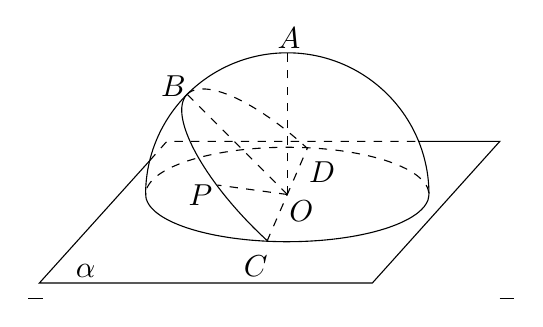
\begin{tikzpicture}[x=1bp,y=-1bp,
  every node/.style={inner sep=0,font=\fontsize{10.5pt}{12.6pt}\selectfont},
  line cap=butt, line join=miter]
  \draw[line width=0.398bp, dash pattern=on 2.989bp off 2.989bp] (162.402,58.168) .. controls (162.402,58.168) and (162.047,56.598) .. (161.754,56.004) .. controls (161.461,55.41) and (160.805,54.461) .. (160.285,53.887) .. controls (159.77,53.309) and (158.758,52.395) .. (158.023,51.848) .. controls (157.285,51.297) and (155.93,50.434) .. (154.992,49.918) .. controls (154.051,49.406) and (152.379,48.609) .. (151.25,48.141) .. controls (150.121,47.668) and (148.156,46.949) .. (146.855,46.531) .. controls (145.559,46.113) and (143.332,45.484) .. (141.883,45.125) .. controls (140.434,44.766) and (137.988,44.234) .. (136.414,43.941) .. controls (134.836,43.645) and (132.207,43.223) .. (130.531,42.996) .. controls (128.859,42.77) and (126.086,42.465) .. (124.34,42.313) .. controls (122.59,42.16) and (119.727,41.977) .. (117.938,41.898) .. controls (116.145,41.82) and (113.234,41.758) .. (111.426,41.758) .. controls (109.621,41.758) and (106.711,41.82) .. (104.918,41.898) .. controls (103.125,41.977) and (100.262,42.16) .. (98.516,42.313) .. controls (96.766,42.465) and (93.996,42.77) .. (92.32,42.996) .. controls (90.645,43.223) and (88.016,43.645) .. (86.441,43.941) .. controls (84.867,44.234) and (82.418,44.766) .. (80.969,45.125) .. controls (79.52,45.484) and (77.297,46.113) .. (75.996,46.531) .. controls (74.695,46.949) and (72.734,47.668) .. (71.605,48.141) .. controls (70.477,48.609) and (68.801,49.406) .. (67.863,49.918) .. controls (66.922,50.434) and (65.566,51.297) .. (64.832,51.848) .. controls (64.098,52.395) and (63.086,53.309) .. (62.566,53.887) .. controls (62.051,54.461) and (61.391,55.41) .. (61.098,56.004) .. controls (60.805,56.598) and (60.453,58.168) .. (60.453,58.168);
  \draw[line width=0.398bp] (162.434,58.762) .. controls (162.434,58.762) and (162.23,60.387) .. (161.984,61.004) .. controls (161.738,61.621) and (161.145,62.605) .. (160.652,63.211) .. controls (160.164,63.809) and (159.184,64.762) .. (158.461,65.336) .. controls (157.738,65.91) and (156.391,66.809) .. (155.445,67.348) .. controls (154.504,67.883) and (152.813,68.719) .. (151.664,69.207) .. controls (150.516,69.699) and (148.508,70.449) .. (147.176,70.887) .. controls (145.844,71.324) and (143.555,71.98) .. (142.063,72.355) .. controls (140.57,72.727) and (138.043,73.277) .. (136.414,73.582) .. controls (134.785,73.887) and (132.063,74.32) .. (130.324,74.551) .. controls (128.59,74.781) and (125.719,75.094) .. (123.906,75.246) .. controls (122.098,75.398) and (119.129,75.578) .. (117.273,75.648) .. controls (115.418,75.723) and (112.402,75.77) .. (110.535,75.762) .. controls (108.668,75.75) and (105.66,75.664) .. (103.816,75.57) .. controls (101.969,75.477) and (99.02,75.262) .. (97.227,75.09) .. controls (95.434,74.914) and (92.594,74.574) .. (90.887,74.32) .. controls (89.176,74.07) and (86.5,73.605) .. (84.906,73.281) .. controls (83.309,72.957) and (80.84,72.379) .. (79.387,71.988) .. controls (77.934,71.598) and (75.719,70.914) .. (74.43,70.465) .. controls (73.145,70.012) and (71.215,69.238) .. (70.121,68.734) .. controls (69.023,68.23) and (67.422,67.379) .. (66.535,66.828) .. controls (65.648,66.281) and (64.395,65.367) .. (63.734,64.785) .. controls (63.07,64.203) and (62.188,63.238) .. (61.766,62.633) .. controls (61.34,62.027) and (60.848,61.035) .. (60.668,60.414) .. controls (60.484,59.797) and (60.453,58.168) .. (60.453,58.168);
  \draw[line width=0.398bp, dash pattern=on 2.989bp off 2.989bp] (75.367,22.699) .. controls (75.367,22.699) and (75.918,22.211) .. (76.152,22.047) .. controls (76.387,21.883) and (76.793,21.648) .. (77.062,21.52) .. controls (77.336,21.395) and (77.797,21.223) .. (78.102,21.133) .. controls (78.406,21.043) and (78.922,20.93) .. (79.258,20.879) .. controls (79.594,20.824) and (80.16,20.773) .. (80.527,20.758) .. controls (80.898,20.746) and (81.512,20.754) .. (81.914,20.777) .. controls (82.312,20.801) and (82.973,20.871) .. (83.402,20.934) .. controls (83.828,20.996) and (84.539,21.125) .. (84.992,21.227) .. controls (85.445,21.324) and (86.195,21.516) .. (86.676,21.652) .. controls (87.156,21.789) and (87.945,22.039) .. (88.453,22.215) .. controls (88.957,22.387) and (89.781,22.695) .. (90.309,22.906) .. controls (90.832,23.113) and (91.695,23.48) .. (92.242,23.723) .. controls (92.789,23.969) and (93.68,24.391) .. (94.242,24.672) .. controls (94.805,24.949) and (95.727,25.43) .. (96.309,25.742) .. controls (96.887,26.055) and (97.832,26.586) .. (98.426,26.93) .. controls (99.02,27.273) and (99.984,27.855) .. (100.59,28.23) .. controls (101.195,28.609) and (102.176,29.238) .. (102.793,29.645) .. controls (103.41,30.051) and (104.406,30.727) .. (105.027,31.16) .. controls (105.652,31.598) and (106.656,32.316) .. (107.285,32.777) .. controls (107.914,33.242) and (108.93,34.004) .. (109.562,34.488) .. controls (110.191,34.977) and (111.207,35.777) .. (111.84,36.285) .. controls (112.473,36.797) and (113.488,37.633) .. (114.121,38.164) .. controls (114.75,38.699) and (115.758,39.566) .. (116.387,40.117) .. controls (117.016,40.668) and (118.637,42.137) .. (118.637,42.137) -- (104.215,75.383);
  \draw[line width=0.398bp] (104.215,75.383) .. controls (104.215,75.383) and (102.312,73.613) .. (101.59,72.922) .. controls (100.871,72.227) and (99.719,71.098) .. (99.016,70.387) .. controls (98.309,69.676) and (97.188,68.52) .. (96.5,67.793) .. controls (95.813,67.066) and (94.727,65.891) .. (94.063,65.156) .. controls (93.398,64.418) and (92.348,63.23) .. (91.711,62.484) .. controls (91.07,61.742) and (90.066,60.543) .. (89.457,59.797) .. controls (88.848,59.051) and (87.891,57.848) .. (87.313,57.102) .. controls (86.738,56.355) and (85.836,55.156) .. (85.293,54.414) .. controls (84.75,53.672) and (83.906,52.484) .. (83.402,51.75) .. controls (82.898,51.016) and (82.121,49.844) .. (81.656,49.121) .. controls (81.191,48.398) and (80.477,47.25) .. (80.055,46.543) .. controls (79.633,45.836) and (78.992,44.711) .. (78.613,44.023) .. controls (78.238,43.332) and (77.668,42.242) .. (77.336,41.578) .. controls (77.008,40.91) and (76.516,39.859) .. (76.23,39.219) .. controls (75.949,38.578) and (75.535,37.57) .. (75.305,36.957) .. controls (75.07,36.348) and (74.738,35.387) .. (74.555,34.809) .. controls (74.375,34.227) and (74.125,33.32) .. (73.996,32.777) .. controls (73.863,32.23) and (73.699,31.383) .. (73.621,30.875) .. controls (73.543,30.367) and (73.461,29.586) .. (73.438,29.117) .. controls (73.414,28.648) and (73.418,27.93) .. (73.445,27.504) .. controls (73.473,27.082) and (73.559,26.43) .. (73.641,26.051) .. controls (73.723,25.672) and (73.895,25.098) .. (74.031,24.762) .. controls (74.164,24.426) and (74.422,23.93) .. (74.605,23.641) .. controls (74.793,23.355) and (75.367,22.699) .. (75.367,22.699);
  \draw[line width=0.398bp] (162.434,58.762) .. controls (162.434,30.59) and (139.598,7.754) .. (111.426,7.754) .. controls (83.258,7.754) and (60.422,30.59) .. (60.422,58.762);
  \draw[line width=0.398bp, dash pattern=on 2.989bp off 2.989bp] (111.426,58.762) -- (111.426,7.754);
  \draw[line width=0.398bp, dash pattern=on 2.989bp off 2.989bp] (111.426,58.762) -- (75.359,22.695);
  \draw[line width=0.398bp, dash pattern=on 2.989bp off 2.989bp] (61.953,46.52) -- (68.07,39.633) -- (158.734,39.633);
  \draw[line width=0.398bp] (61.953,46.52) -- (22.168,90.641) -- (142.031,90.641) -- (187.934,39.633) -- (158.734,39.633);
  \draw[line width=0.398bp, dash pattern=on 2.989bp off 2.989bp] (111.426,58.762) -- (86.266,55.359);
  \draw[line width=0.42bp] (18.176,96.277) -- (23.426,96.277);
  \draw[line width=0.42bp] (187.895,96.277) -- (193.145,96.277);
  \node[anchor=base west] at (107.72,6.16) {$A$};
  \node[anchor=base west] at (65.82,23.54) {$B$};
  \node[anchor=base west] at (119.07,54.27) {$D$};
  \node[anchor=base west] at (75.75,62.77) {$P$};
  \node[anchor=base west] at (111.95,68.36) {$O$};
  \node[anchor=base west] at (95.62,88.28) {$C$};
  \node[anchor=base west] at (35.14,88.66) {$\alpha$};
\end{tikzpicture}
\end{center}
\nopagebreak[4]
（A）$R\arccos\dfrac{\sqrt2}{4}$；（B）$\dfrac{\pi R}{4}$；（C）$R\arccos\dfrac{\sqrt3}{3}$；（D）$\dfrac{\pi R}{3}$。

\Needspace{4\baselineskip}
\textbf{解析}

以 $O$ 为原点、平面 $\alpha$ 为 $xOy$ 平面、$OA$ 为 $z$ 轴，则 $A(0,0,R)$。

\Needspace{5\baselineskip}
平面 $\alpha$ 与过 $CD$ 的 $45^\circ$ 平面的交线即 $CD$（取为 $y$ 轴）。该 $45^\circ$ 平面与半球面的交线是半圆，其上到 $\alpha$ 距离最大（$z$ 最大）的点 $B$ 位于 $yOz$ 平面内，且 $\angle BOC=45^\circ$，故
\nopagebreak[4]
\[B\left(0,\ -R\cos45^\circ,\ R\sin45^\circ\right)=\left(0,\ -\frac{\sqrt2}2R,\ \frac{\sqrt2}2R\right).\]

\Needspace{5\baselineskip}
$P$ 在该半圆上且 $\angle BOP=60^\circ$。以 $\boldsymbol e=(1,0,0)$ 记半圆所在平面内与 $OB$ 垂直的单位向量，则
\nopagebreak[4]
\[P=R\left(\sin60^\circ\right)\boldsymbol e+R\left(\cos60^\circ\right)\frac{B}{R},\]
\nopagebreak[4]
\[P=\left(\frac{\sqrt3}2R,\ -\frac{\sqrt2}4R,\ \frac{\sqrt2}4R\right).\]
\Needspace{5\baselineskip}
于是
\nopagebreak[4]
\[\overrightarrow{OA}\cdot\overrightarrow{OP}=0+0+R\cdot\frac{\sqrt2}4R=\frac{\sqrt2}4R^2,\]
\nopagebreak[4]
\[\cos\angle AOP=\frac{\overrightarrow{OA}\cdot\overrightarrow{OP}}{|OA||OP|}=\frac{\sqrt2}4.\]
故 $A$，$P$ 的球面距离为 $R\arccos\dfrac{\sqrt2}4$。选 A。

\gkanswer{答案：A。}

\end{answer}
\begin{answer}
\gksolhead{11}{}

\textbf{题目}：

方程 $ay=b^2x^2+c$ 中的 $a$，$b$，$c\in\{-3,-2,0,1,2,3\}$，且 $a$，$b$，$c$ 互不相同，在所有这些方程所表示的曲线中，不同的抛物线共有\mbox{（　　）}

（A）$60$ 条；（B）$62$ 条；（C）$71$ 条；（D）$80$ 条。

\Needspace{4\baselineskip}
\textbf{解析}

\Needspace{5\baselineskip}
方程 $ay=b^2x^2+c$ 表示抛物线需 $a\neq0$ 且 $b\neq0$（$b=0$ 时化为 $y=\dfrac ca$，是直线）。化简为
\nopagebreak[4]
\[y=\frac{b^2}ax^2+\frac ca,\]
故两条方程表示同一条抛物线当且仅当 $\dfrac{b^2}a$ 与 $\dfrac ca$ 都相同。

\Needspace{5\baselineskip}
计数：$a\neq0$ 有 $5$ 种取法（从 $\{-3,-2,0,1,2,3\}$ 去掉 $0$），$b$ 从剩余 $5$ 个数中取，$c$ 从剩余 $4$ 个数中取，共 $5\times5\times4=100$ 个方程。其中 $b=0$ 的有 $5\times4=20$ 个（退化为直线，不是抛物线），剩下
\nopagebreak[4]
\[100-20=80\]
个方程对应抛物线。

\Needspace{5\baselineskip}
去重：当 $b$ 与 $-b$ 同时可选时，二者给出相同的 $\dfrac{b^2}a$，而 $c$ 的可选集合也完全一致，故每对 $\pm b$ 使同一抛物线被计两次。枚举 $b=\pm2$，$\pm3$ 的各类组合，重复计数共 $18$ 对，因此不同的抛物线有
\nopagebreak[4]
\[80-18=62\ \text{\text{条}}.\]

选 B。

\gkanswer{答案：B。}

\end{answer}
\begin{answer}
\gksolhead{12}{}

\textbf{题目}：

设函数 $f(x)=2x-\cos x$，$\{a_n\}$ 是公差为 $\dfrac\pi8$ 的等差数列，$f(a_1)+f(a_2)+\cdots+f(a_5)=5\pi$，则 $[f(a_3)]^2-a_1a_5=$\mbox{（　　）}

（A）$0$；（B）$\dfrac1{16}\pi^2$；（C）$\dfrac18\pi^2$；（D）$\dfrac{13}{16}\pi^2$。

\Needspace{4\baselineskip}
\textbf{解析}

\Needspace{5\baselineskip}
设公差 $d=\dfrac\pi8$，$a_3=t$，则 $a_i=t+(i-3)d$（$i=1,2,\cdots,5$）。由
\nopagebreak[4]
\[\sum_{i=1}^5f(a_i)=2\sum_{i=1}^5a_i-\sum_{i=1}^5\cos a_i=10t-\sum_{k=-2}^{2}\cos(t+kd).\]
\Needspace{5\baselineskip}
利用和差化积，
\nopagebreak[4]
\[\sum_{k=-2}^{2}\cos(t+kd)=\cos t\left(1+2\cos d+2\cos2d\right).\]
取 $t=\dfrac\pi2$：$\cos t=0$ 使第二项为零，第一项 $10\cdot\dfrac\pi2=5\pi$，故 $t=\dfrac\pi2$ 满足条件（$f$ 单调，解唯一）。

\Needspace{5\baselineskip}
于是 $a_3=\dfrac\pi2$，$f(a_3)=2\cdot\dfrac\pi2-\cos\dfrac\pi2=\pi$，且
\nopagebreak[4]
\[a_1a_5=\left(a_3-2d\right)\left(a_3+2d\right)=a_3^2-4d^2=\frac{\pi^2}4-\frac{\pi^2}{16}=\frac{3\pi^2}{16}.\]
\Needspace{5\baselineskip}
故
\nopagebreak[4]
\[[f(a_3)]^2-a_1a_5=\pi^2-\frac{3\pi^2}{16}=\frac{13\pi^2}{16}.\]
选 D。

\gkanswer{答案：D。}

\end{answer}
\begin{answer}
\gksolhead{13}{}

\textbf{题目}：

设全集 $U=\{a,b,c,d\}$，集合 $A=\{a,b\}$，$B=\{b,c,d\}$，则 $\complement_U A\cup\complement_U B=$\gkblank{}。

\Needspace{4\baselineskip}
\textbf{解析}

\Needspace{5\baselineskip}
$A\cup B=\{a,b\}\cup\{b,c,d\}=\{a,b,c,d\}=U$，故
\nopagebreak[4]
\[\complement_UA=\left\{c,d\right\},\qquad \complement_UB=\left\{a\right\},\]
\nopagebreak[4]
\[\complement_UA\cup\complement_UB=\{a,c,d\}.\]

\gkanswer{答案：$\{a,c,d\}$。}

\end{answer}
\begin{answer}
\gksolhead{14}{}

\textbf{题目}：

如图，在正方体 $ABCD-A_1B_1C_1D_1$ 中，$M$，$N$ 分别是 $CD$，$CC_1$ 的中点，则异面直线 $A_1M$ 与 $DN$ 所成角的大小是\gkblank{}。
\nopagebreak[4]
\begin{center}%% ============================================================
% f2012_sichuan_sci_q14_cube.tex
%% 2012 四川卷（理科）第 14 题 正方体 ABCD-A1B1C1D1，M、N 分别为 CD、CC1 的中点
%% 来源 PDF：普通高考/2012/2012四川理.pdf 第 1 页（印面 771）第 3 栏
%% 坐标取自原页矢量层（bp），原点为图区左上角 (908.0,55.0)，y 向下；虚线照原页。
%% ============================================================
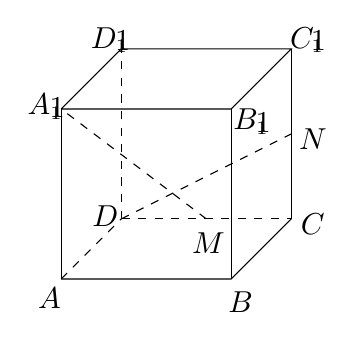
\begin{tikzpicture}[x=1bp,y=-1bp,
  every node/.style={inner sep=0,font=\fontsize{10.5pt}{12.6pt}\selectfont},
  line cap=butt, line join=miter]
  \draw[line width=0.398bp] (17.738,97.422) -- (78.945,97.422) -- (100.582,75.785);
  \draw[line width=0.398bp] (17.738,36.215) -- (78.945,36.215) -- (100.582,14.574) -- (39.375,14.574) -- (17.738,36.215);
  \draw[line width=0.398bp] (78.945,97.422) -- (78.945,36.211);
  \draw[line width=0.398bp] (100.586,75.785) -- (100.586,14.574);
  \draw[line width=0.398bp] (17.738,97.422) -- (17.738,36.211);
  \draw[line width=0.398bp, dash pattern=on 2.989bp off 2.989bp] (17.738,97.422) -- (39.375,75.785);
  \draw[line width=0.398bp, dash pattern=on 2.989bp off 2.989bp] (39.375,75.785) -- (100.586,75.785);
  \draw[line width=0.398bp, dash pattern=on 2.989bp off 2.989bp] (39.375,75.785) -- (39.375,14.574);
  \draw[line width=0.398bp, dash pattern=on 2.989bp off 2.989bp] (69.98,75.785) -- (17.738,36.215);
  \draw[line width=0.398bp, dash pattern=on 2.989bp off 2.989bp] (39.375,75.785) -- (100.586,45.18);
  \node[anchor=base west] at (28.22,14.4) {$D_1$};
  \node[anchor=base west] at (36.91,15.29) {$1$};
  \node[anchor=base west] at (99.91,14.4) {$C_1$};
  \node[anchor=base west] at (107.41,15.29) {$1$};
  \node[anchor=base west] at (5.47,38.31) {$A_1$};
  \node[anchor=base west] at (13.35,39.2) {$1$};
  \node[anchor=base west] at (79.55,43.65) {$B_1$};
  \node[anchor=base west] at (87.51,44.54) {$1$};
  \node[anchor=base west] at (103.15,50.74) {$N$};
  \node[anchor=base west] at (28.8,78.69) {$D$};
  \node[anchor=base west] at (103.81,81.35) {$C$};
  \node[anchor=base west] at (64.68,88.33) {$M$};
  \node[anchor=base west] at (9.22,107.93) {$A$};
  \node[anchor=base west] at (77.74,109.44) {$B$};
\end{tikzpicture}
\end{center}
\nopagebreak[4]
\Needspace{4\baselineskip}
\textbf{解析}

\Needspace{5\baselineskip}
以 $D$ 为原点，$DA$，$DC$，$DD_1$ 为坐标轴，取棱长为 $2$，则
\nopagebreak[4]
\[D(0,0,0),\quad A_1(2,0,2),\quad M(0,1,0),\quad N(0,2,1).\]
\Needspace{5\baselineskip}
故
\nopagebreak[4]
\[\overrightarrow{A_1M}=(-2,1,-2),\qquad \overrightarrow{DN}=(0,2,1),\]
\nopagebreak[4]
\[\overrightarrow{A_1M}\cdot\overrightarrow{DN}=0+2-2=0.\]
所以 $A_1M\perp DN$，异面直线 $A_1M$ 与 $DN$ 所成角为 $90^\circ$。

\gkanswer{答案：$90^\circ$。}

\end{answer}
\begin{answer}
\gksolhead{15}{}

\textbf{题目}：

椭圆 $\dfrac{x^2}4+\dfrac{y^2}3=1$ 的左焦点为 $F$，直线 $x=m$ 与椭圆相交于点 $A$，$B$，当 $\triangle FAB$ 的周长最大时，$\triangle FAB$ 的面积是\gkblank{}。

\Needspace{4\baselineskip}
\textbf{解析}

由椭圆方程知 $a=2$，$b=\sqrt3$，$c=\sqrt{a^2-b^2}=1$，故左焦点 $F(-1,0)$。

\Needspace{5\baselineskip}
设 $A(m,y)$，$B(m,-y)$（$y>0$），则 $y^2=3\left(1-\dfrac{m^2}4\right)$，且
\nopagebreak[4]
\[|AF|=|BF|=\sqrt{(m+1)^2+y^2}.\]
\Needspace{5\baselineskip}
周长
\nopagebreak[4]
\[L(m)=2y+2\sqrt{(m+1)^2+y^2},\qquad -2<m<2.\]
\Needspace{5\baselineskip}
求导并令其为零：
\nopagebreak[4]
\[L'(m)=2y'+2\cdot\frac{(m+1)+yy'}{\sqrt{(m+1)^2+y^2}}=0,\]
\Needspace{5\baselineskip}
其中 $y'=-\dfrac{m}{4y}\cdot3=-\dfrac{3m}{4y}$。代入化简可得唯一驻点 $m=1$，此时 $y=\dfrac32$、$L(1)=8$；而端点 $L(-2)=2$、$L(2)=6$，驻点处确为最大值。故
\nopagebreak[4]
\[L_{\max}=L(1)=3+2\sqrt{4+\frac94}=3+5=8.\]
\Needspace{5\baselineskip}
此时
\nopagebreak[4]
\[S_{\triangle FAB}=\frac12|AB|\cdot d(F,\text{\text{直线} }x=m)=\frac12\cdot2y\cdot|m+1|=\frac32\cdot2=3.\]

\gkanswer{答案：$3$。}

\end{answer}
\begin{answer}
\gksolhead{16}{}

\textbf{题目}：

记 $[x]$ 为不超过实数 $x$ 的最大整数，例如，$[2]=2$，$[1.5]=1$，$[-0.3]=-1$。

设 $a$ 为正整数，数列 $\{x_n\}$ 满足 $x_1=a$，$x_{n+1}=\left[\dfrac{x_n+\dfrac{a}{x_n}}{2}\right]$（$n\in\mathbf N^*$）。现有下列命题：

① 当 $a=5$ 时，数列 $\{x_n\}$ 的前 $3$ 项依次为 $5$，$3$，$2$；

② 对数列 $\{x_n\}$ 都存在正整数 $k$，当 $n\geqslant k$ 时总有 $x_n=x_k$；

③ 当 $n\geqslant1$ 时，$x_n>\sqrt a-1$；

④ 对某个正整数 $k$，若 $x_{k+1}\geqslant x_k$，则 $x_n=[\sqrt a]$。

其中的真命题有\gkblank{}。（写出所有真命题的编号）

\Needspace{4\baselineskip}
\textbf{解析}

\Needspace{5\baselineskip}
① 直接迭代。$a=5$：$x_1=5$，
\nopagebreak[4]
\[x_2=\left[\frac{5+\frac55}{2}\right]=[3]=3,\qquad x_3=\left[\frac{3+\frac53}{2}\right]=\left[\frac73\right]=2.\]
故前 $3$ 项依次为 $5$，$3$，$2$，真。

② 假。取 $a=3$：$x_1=3$，$x_2=[2]=2$，$x_3=\left[\dfrac{2+\frac32}2\right]=[1.75]=1$，$x_4=\left[\dfrac{1+3}2\right]=2$，此后 $1,2,1,2,\cdots$ 循环，不趋于常值，故不存在这样的 $k$。

\Needspace{5\baselineskip}
③ 真。$a$ 是正整数，故 $a\geqslant1$，$x_1=a\geqslant[\sqrt a]$。又由均值不等式，对 $x>0$ 有
\nopagebreak[4]
\[\frac{x_n+\frac a{x_n}}2\geqslant\sqrt a,\]
\Needspace{5\baselineskip}
故
\nopagebreak[4]
\[x_{n+1}=\left[\frac{x_n+\frac a{x_n}}2\right]\geqslant\left[\sqrt a\right].\]
\Needspace{5\baselineskip}
于是对一切 $n\geqslant1$ 都有 $x_n\geqslant[\sqrt a]$。而由取整函数的定义
\nopagebreak[4]
\[[\sqrt a]>\sqrt a-1,\]
故 $x_n>\sqrt a-1$。

④ 假。仍取 $a=3$，数列为 $3,2,1,2,1,2,\cdots$。取 $k=3$，有 $x_4=2\geqslant x_3=1$，但数列并不恒等于 $[\sqrt3]=1$（$x_4=2$），故命题不成立。

故真命题为 ①③。

\gkanswer{答案：①③。}

\end{answer}
\begin{answer}
\gksolhead{17}{}

\textbf{题目}：

某居民小区有两个相互独立的安全防范系统（简称系统）$A$ 和 $B$，系统 $A$ 和 $B$ 在任意时刻发生故障的概率分别为 $\dfrac1{10}$ 和 $p$。

（1） 若在任意时刻至少有一个系统不发生故障的概率为 $\dfrac{49}{50}$，求 $p$ 的值；

（2） 设系统 $A$ 在 $3$ 次相互独立的检测中不发生故障的次数为随机变量 $\xi$，求 $\xi$ 的概率分布列及数学期望 $E\xi$。

\Needspace{4\baselineskip}
\textbf{解析}

\textbf{（1）} 记系统 $A$，$B$ 发生故障分别为事件 $E_A$，$E_B$，$P(E_A)=\dfrac1{10}$，$P(E_B)=p$，二者相互独立。

\Needspace{5\baselineskip}
「至少有一个系统不发生故障」的对立事件是「两个系统都发生故障」，故
\nopagebreak[4]
\[1-P(E_A)P(E_B)=1-\frac p{10}=\frac{49}{50}.\]
于是 $\dfrac p{10}=\dfrac1{50}$，得 $p=\dfrac15$。

\Needspace{5\baselineskip}
\textbf{（2）} 系统 $A$ 每次检测不发生故障的概率为 $\dfrac9{10}$，各次检测相互独立，故
\nopagebreak[4]
\[\xi\sim B\left(3,\frac9{10}\right),\]
\nopagebreak[4]
\[P(\xi=k)=\mathrm C_3^k\left(\frac9{10}\right)^k\left(\frac1{10}\right)^{3-k},\qquad k=0,1,2,3.\]
\Needspace{5\baselineskip}
逐一计算：
\nopagebreak[4]
\[P(\xi=0)=\frac1{1000},\qquad P(\xi=1)=\frac{3\times9}{1000}=\frac{27}{1000},\]
\nopagebreak[4]
\[P(\xi=2)=\frac{3\times81}{1000}=\frac{243}{1000},\qquad P(\xi=3)=\frac{729}{1000}.\]
\Needspace{5\baselineskip}
数学期望
\nopagebreak[4]
\[E\xi=3\times\frac9{10}=\frac{27}{10}.\]

\gkanswer{答案（1）：$p=\dfrac15$。}

\gkanswer{答案（2）：$\xi$ 的分布列为 $P(\xi=0)=\dfrac1{1000}$，$P(\xi=1)=\dfrac{27}{1000}$，$P(\xi=2)=\dfrac{243}{1000}$，$P(\xi=3)=\dfrac{729}{1000}$；$E\xi=\dfrac{27}{10}$。}

\end{answer}
\begin{answer}
\gksolhead{18}{}

\textbf{题目}：

函数 $f(x)=6\cos^2\dfrac{\omega x}{2}+\sqrt3\sin\omega x-3$（$\omega>0$）在一个周期内的图象如图所示，$A$ 为图象的最高点，$B$，$C$ 为图象与 $x$ 轴的交点，且 $\triangle ABC$ 为正三角形。

（1） 求 $\omega$ 的值及函数 $f(x)$ 的值域；

（2） 若 $f(x_0)=\dfrac{8\sqrt3}{5}$，且 $x_0\in\left(-\dfrac{10}3,\dfrac23\right)$，求 $f(x_0+1)$ 的值。
\nopagebreak[4]
\begin{center}%% ============================================================
% f2012_sichuan_sci_q18_wave.tex
%% 2012 四川卷（理科）第 18 题 f(x) 在一个周期内的图象，A 为最高点，B、C 为图象与 x 轴交点
%% 来源 PDF：普通高考/2012/2012四川理.pdf 第 2 页（印面 772）第 1 栏
%% 坐标取自原页矢量层（bp），原点为图区左上角 (230.0,160.0)，y 向下；AB、AC 为原页实线。
%% ============================================================
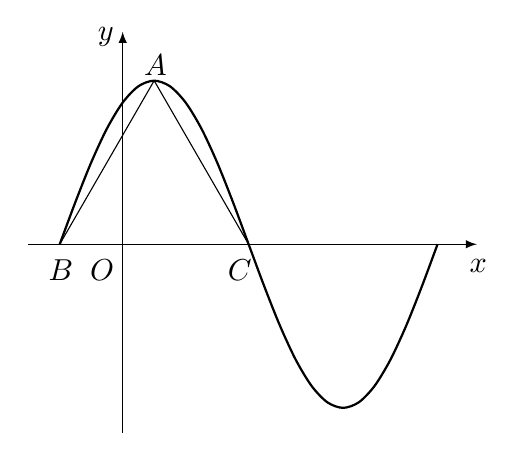
\begin{tikzpicture}[x=1bp,y=-1bp,
  every node/.style={inner sep=0,font=\fontsize{10.5pt}{12.6pt}\selectfont},
  line cap=butt, line join=miter]
  \draw[line width=0.3985bp] (6.215,85.234) -- (164.148,85.234);
  \fill[black] (167.734,85.234) .. controls (166.672,85.035) and (164.945,84.438) .. (163.75,83.738) -- (163.75,86.727) .. controls (164.945,86.031) and (166.672,85.434) .. (167.734,85.234);
  \draw[line width=0.3985bp] (40.219,153.242) -- (40.219,12.309);
  \fill[black] (40.219,8.727) .. controls (40.02,9.789) and (39.422,11.516) .. (38.727,12.707) -- (41.711,12.707) .. controls (41.016,11.516) and (40.418,9.789) .. (40.219,8.727);
  \draw[line width=0.797bp] (17.551,85.234) .. controls (17.551,85.234) and (21.645,74.074) .. (23.219,69.988) .. controls (24.789,65.902) and (27.313,59.449) .. (28.883,55.785) .. controls (30.457,52.121) and (32.98,46.578) .. (34.551,43.59) .. controls (36.125,40.598) and (38.645,36.344) .. (40.219,34.23) .. controls (41.793,32.113) and (44.313,29.441) .. (45.887,28.348) .. controls (47.457,27.25) and (49.98,26.34) .. (51.555,26.34) .. controls (53.125,26.34) and (55.648,27.25) .. (57.219,28.344) .. controls (58.793,29.438) and (61.316,32.113) .. (62.887,34.227) .. controls (64.461,36.34) and (66.98,40.594) .. (68.555,43.586) .. controls (70.129,46.578) and (72.648,52.121) .. (74.223,55.781) .. controls (75.793,59.445) and (78.316,65.902) .. (79.891,69.988) .. controls (81.461,74.07) and (83.984,81) .. (85.555,85.23) .. controls (87.129,89.457) and (89.652,96.387) .. (91.223,100.469) .. controls (92.797,104.555) and (95.316,111.012) .. (96.891,114.676) .. controls (98.465,118.34) and (100.984,123.883) .. (102.559,126.875) .. controls (104.129,129.863) and (106.652,134.117) .. (108.227,136.234) .. controls (109.797,138.352) and (112.32,141.023) .. (113.891,142.121) .. controls (115.465,143.215) and (117.988,144.129) .. (119.559,144.129) .. controls (121.133,144.129) and (123.652,143.219) .. (125.227,142.125) .. controls (126.801,141.031) and (129.32,138.355) .. (130.895,136.242) .. controls (132.465,134.129) and (134.988,129.875) .. (136.562,126.883) .. controls (138.133,123.895) and (140.656,118.352) .. (142.227,114.691) .. controls (143.801,111.027) and (146.324,104.57) .. (147.895,100.484) .. controls (149.469,96.398) and (153.562,85.242) .. (153.562,85.242);
  \draw[line width=0.3985bp] (17.551,85.234) -- (51.555,26.336) (51.555,26.336) -- (85.559,85.234);
  \node[anchor=base west] at (31.1,11.96) {$y$};
  \node[anchor=base west] at (47.72,24.64) {$A$};
  \node[anchor=base west] at (164.88,95.48) {$x$};
  \node[anchor=base west] at (13.4,98.13) {$B$};
  \node[anchor=base west] at (28.32,98.13) {$O$};
  \node[anchor=base west] at (77.86,98.13) {$C$};
\end{tikzpicture}
\end{center}
\nopagebreak[4]
\Needspace{4\baselineskip}
\textbf{解析}

\Needspace{5\baselineskip}
\textbf{（1）} 由二倍角公式，
\nopagebreak[4]
\[f(x)=3\left(1+\cos\omega x\right)+\sqrt3\sin\omega x-3=3\cos\omega x+\sqrt3\sin\omega x,\]
\Needspace{5\baselineskip}
即
\nopagebreak[4]
\[f(x)=2\sqrt3\sin\left(\omega x+\frac\pi3\right).\]
故值域为 $\left[-2\sqrt3,\ 2\sqrt3\right]$，周期 $T=\dfrac{2\pi}\omega$。

\Needspace{5\baselineskip}
$\triangle ABC$ 为正三角形，$A$ 为最高点，$B$，$C$ 为相邻两个零点，故 $|BC|=\dfrac T2=\dfrac\pi\omega$，高为 $2\sqrt3$。由正三角形的高与边长关系
\nopagebreak[4]
\[2\sqrt3=\frac{\sqrt3}2\cdot\frac\pi\omega\ \Longrightarrow\ \omega=\frac\pi4.\]
所以 $\omega=\dfrac\pi4$，$f(x)$ 的值域为 $\left[-2\sqrt3,\ 2\sqrt3\right]$。

\Needspace{5\baselineskip}
\textbf{（2）} 由 $f(x_0)=\dfrac{8\sqrt3}5$ 得
\nopagebreak[4]
\[2\sqrt3\sin\left(\frac\pi4x_0+\frac\pi3\right)=\frac{8\sqrt3}5,\]
\nopagebreak[4]
\[\sin\left(\frac\pi4x_0+\frac\pi3\right)=\frac45.\]
\Needspace{5\baselineskip}
由 $x_0\in\left(-\dfrac{10}3,\dfrac23\right)$ 得 $\dfrac\pi4x_0+\dfrac\pi3\in\left(-\dfrac\pi2,\dfrac\pi2\right)$，故
\nopagebreak[4]
\[\cos\left(\frac\pi4x_0+\frac\pi3\right)=\frac35.\]
\Needspace{5\baselineskip}
于是
\nopagebreak[4]
\[f(x_0+1)=2\sqrt3\sin\left(\frac\pi4x_0+\frac\pi3+\frac\pi4\right),\]
\nopagebreak[4]
\[f(x_0+1)=2\sqrt3\left(\frac45\cdot\frac{\sqrt2}2+\frac35\cdot\frac{\sqrt2}2\right)=\frac{7\sqrt6}5.\]

\gkanswer{答案（1）：$\omega=\dfrac\pi4$，值域 $\left[-2\sqrt3,\ 2\sqrt3\right]$。}

\gkanswer{答案（2）：$\dfrac{7\sqrt6}{5}$。}

\end{answer}
\begin{answer}
\gksolhead{19}{}

\textbf{题目}：

如图，在三棱锥 $P-ABC$ 中，$\angle APB=90^\circ$，$\angle PAB=60^\circ$，$AB=BC=CA$，平面 $PAB\perp$ 平面 $ABC$。

（1） 求直线 $PC$ 与平面 $ABC$ 所成角的正弦值；

（2） 求二面角 $B-AP-C$ 的余弦值。
\nopagebreak[4]
\begin{center}%% ============================================================
% f2012_sichuan_sci_q19_pyramid.tex
%% 2012 四川卷（理科）第 19 题 三棱锥 P-ABC，∠APB=90°，∠PAB=60°，平面PAB⊥平面ABC
%% 来源 PDF：普通高考/2012/2012四川理.pdf 第 2 页（印面 772）第 1 栏
%% 坐标取自原页矢量层（bp），原点为图区左上角 (230.0,525.0)，y 向下；虚线照原页。
%% ============================================================
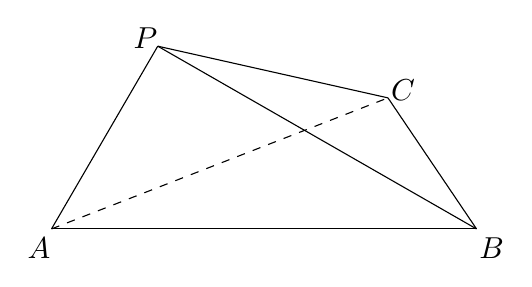
\begin{tikzpicture}[x=1bp,y=-1bp,
  every node/.style={inner sep=0,font=\fontsize{10.5pt}{12.6pt}\selectfont},
  line cap=butt, line join=miter]
  \draw[line width=0.3985bp] (8.547,74.539) -- (161.559,74.539);
  \draw[line width=0.3985bp] (161.559,74.539) -- (129.68,27.359);
  \draw[line width=0.3985bp] (129.68,27.359) -- (46.801,8.746);
  \draw[line width=0.3985bp] (46.801,8.746) -- (8.547,74.539);
  \draw[line width=0.3985bp] (46.801,8.746) -- (161.559,74.539);
  \draw[line width=0.3985bp, dash pattern=on 2.989bp off 2.989bp] (8.547,74.539) -- (129.68,27.359);
  \node[anchor=base west] at (37.87,9.54) {$P$};
  \node[anchor=base west] at (130.62,28.16) {$C$};
  \node[anchor=base west] at (-0.23,85.22) {$A$};
  \node[anchor=base west] at (162.39,85.22) {$B$};
\end{tikzpicture}
\end{center}
\nopagebreak[4]
\Needspace{4\baselineskip}
\textbf{解析}

\Needspace{5\baselineskip}
\textbf{（1）} 设 $AB=BC=CA=2$。由 $\angle APB=90^\circ$，$\angle PAB=60^\circ$ 得 $\angle PBA=30^\circ$，故
\nopagebreak[4]
\[AP=AB\sin30^\circ=1,\qquad AO=AP\cos60^\circ=\frac12,\qquad PO=AP\sin60^\circ=\frac{\sqrt3}2.\]
$O$ 是 $P$ 在平面 $ABC$ 上的射影，故 $PO\perp$ 平面 $ABC$，$\angle PCO$ 即直线 $PC$ 与平面 $ABC$ 所成的角。

\Needspace{5\baselineskip}
在正 $\triangle ABC$ 中 $AC=2$，$AO=\dfrac12$，$\angle BAC=60^\circ$，由余弦定理
\nopagebreak[4]
\[CO^2=AC^2+AO^2-2\cdot AC\cdot AO\cos60^\circ=4+\frac14-1=\frac{13}4.\]
\Needspace{5\baselineskip}
而 $PO\perp CO$，故
\nopagebreak[4]
\[PC^2=PO^2+CO^2=\frac34+\frac{13}4=4,\qquad PC=2.\]
\Needspace{5\baselineskip}
于是
\nopagebreak[4]
\[\sin\angle PCO=\frac{PO}{PC}=\frac{\frac{\sqrt3}2}2=\frac{\sqrt3}4.\]

\Needspace{5\baselineskip}
\textbf{（2）} 以 $A$ 为原点，$AB$ 为 $x$ 轴、平面 $ABC$ 为 $xOy$ 平面建立坐标系，取 $AB=2$，则
\nopagebreak[4]
\[A(0,0,0),\quad B(2,0,0),\quad C\left(1,\sqrt3,0\right),\quad O\left(\frac12,0,0\right),\quad P\left(\frac12,0,\frac{\sqrt3}2\right).\]

平面 $BAP$ 即 $xOz$ 平面，取其法向量 $\boldsymbol n_1=(0,1,0)$。

\Needspace{5\baselineskip}
平面 $CAP$ 的法向量
\nopagebreak[4]
\[\boldsymbol n_2=\overrightarrow{AC}\times\overrightarrow{AP}=\left(1,\sqrt3,0\right)\times\left(\frac12,0,\frac{\sqrt3}2\right)=\left(\frac32,-\frac{\sqrt3}2,-\frac{\sqrt3}2\right).\]
\Needspace{5\baselineskip}
于是
\nopagebreak[4]
\[\cos\theta=\frac{\left|\boldsymbol n_1\cdot\boldsymbol n_2\right|}{|\boldsymbol n_1||\boldsymbol n_2|}=\frac{\frac{\sqrt3}2}{1\cdot\sqrt{\frac94+\frac34+\frac34}}=\frac{\frac{\sqrt3}2}{\sqrt3\cdot\frac{\sqrt5}2}=\frac1{\sqrt5}=\frac{\sqrt5}5.\]

\gkanswer{答案（1）：$\dfrac{\sqrt3}4$。}

\gkanswer{答案（2）：$\dfrac{\sqrt5}5$。}

\end{answer}
\begin{answer}
\gksolhead{20}{}

\textbf{题目}：

已知数列 $\{a_n\}$ 的前 $n$ 项和为 $S_n$，且 $a_2a_n=S_2+S_n$ 对一切正整数 $n$ 都成立。

（1） 求 $a_1$，$a_2$ 的值；

（2） 设 $a_1>0$，数列 $\left\{\lg\dfrac{10a_1}{a_n}\right\}$ 的前 $n$ 项和为 $T_n$，当 $n$ 为何值时，$T_n$ 最大？并求出 $T_n$ 的最大值。

\Needspace{4\baselineskip}
\textbf{解析}

\textbf{（1）} 取 $n=1$：$a_2a_1=S_2+S_1=2a_1+a_2$；取 $n=2$：$a_2^2=S_2+S_2=2\left(a_1+a_2\right)$。

\Needspace{5\baselineskip}
由第一式得 $a_2(a_1-1)=2a_1$，即 $a_2=\dfrac{2a_1}{a_1-1}$（$a_1\neq1$）。代入第二式：
\nopagebreak[4]
\[\frac{4a_1^2}{(a_1-1)^2}=2a_1+\frac{4a_1}{a_1-1}.\]
\Needspace{5\baselineskip}
两边乘以 $\dfrac{(a_1-1)^2}{2a_1}$（$a_1\neq0$）：
\nopagebreak[4]
\[2a_1=(a_1-1)^2+2(a_1-1)=a_1^2-1,\]
\Needspace{5\baselineskip}
即 $a_1^2-2a_1-1=0$，解得 $a_1=1\pm\sqrt2$，对应
\nopagebreak[4]
\[a_2=2\pm\sqrt2\quad(\text{\text{同号取}}).\]
另有 $a_1=0$：此时 $a_2\cdot0=S_2+0=a_2$ 迫使 $a_2=0$，故 $(0,0)$ 也是解。

所以 $(a_1,a_2)=(0,0)$，或 $(1+\sqrt2,2+\sqrt2)$，或 $(1-\sqrt2,2-\sqrt2)$。

\Needspace{5\baselineskip}
\textbf{（2）} 一般地，由 $a_2a_n=S_2+S_n$ 与 $a_2a_{n-1}=S_2+S_{n-1}$（$n\geqslant2$）相减得
\nopagebreak[4]
\[a_2\left(a_n-a_{n-1}\right)=a_n,\]
\Needspace{5\baselineskip}
即 $a_n\left(a_2-1\right)=a_2a_{n-1}$。$a_1>0$ 时 $a_1=1+\sqrt2$，$a_2=2+\sqrt2$，$a_2-1=1+\sqrt2$，故公比
\nopagebreak[4]
\[q=\frac{a_2}{a_2-1}=\frac{2+\sqrt2}{1+\sqrt2}=\sqrt2,\]
从而 $a_n=a_1\left(\sqrt2\right)^{n-1}$。

\Needspace{5\baselineskip}
由 $a_n>0$ 得
\nopagebreak[4]
\[\lg\frac{10a_1}{a_n}=\lg10+\lg a_1-\lg a_n=1+\lg a_1-\lg a_n,\]
\Needspace{5\baselineskip}
前 $n$ 项和
\nopagebreak[4]
\[T_n=n\left(1+\lg a_1\right)-\sum_{k=1}^n\lg a_k.\]
\Needspace{5\baselineskip}
而 $\lg a_k=\lg a_1+(k-1)\lg\sqrt2=\lg a_1+(k-1)\cdot\dfrac{\lg2}2$，故
\nopagebreak[4]
\[T_n=n-\frac{\lg2}2\cdot\frac{n(n-1)}2=n-\frac{\lg2}4n(n-1).\]
\Needspace{5\baselineskip}
这是关于 $n$ 的二次函数，开口向下，对称轴
\nopagebreak[4]
\[n=\frac{1+\frac{\lg2}4}{2\cdot\frac{\lg2}4}\approx7.14,\]
\Needspace{5\baselineskip}
故 $n=7$ 时 $T_n$ 最大，
\nopagebreak[4]
\[T_7=7-\frac{\lg2}4\cdot42=7-\frac{21}2\lg2.\]

\gkanswer{答案（1）：$a_1=a_2=0$，或 $a_1=1+\sqrt2$、$a_2=2+\sqrt2$，或 $a_1=1-\sqrt2$、$a_2=2-\sqrt2$。}

\gkanswer{答案（2）：$n=7$ 时 $T_n$ 最大，$T_7=7-\dfrac{21}2\lg2$。}

\end{answer}
\begin{answer}
\gksolhead{21}{}

\textbf{题目}：

如图，动点 $M$ 与两定点 $A(-1,0)$，$B(2,0)$ 构成 $\triangle MAB$，且 $\angle MBA=2\angle MAB$，设动点 $M$ 的轨迹为 $C$。

（1） 求轨迹 $C$ 的方程；

（2） 设直线 $y=-2x+m$ 与 $y$ 轴相交于点 $P$，与轨迹 $C$ 相交于点 $Q$、$R$，且 $|PQ|<|PR|$，求 $\dfrac{|PR|}{|PQ|}$ 的取值范围。
\nopagebreak[4]
\begin{center}%% ============================================================
% f2012_sichuan_sci_q21_locus.tex
%% 2012 四川卷（理科）第 21 题 动点 M 与定点 A(-1,0)、B(2,0)，∠MBA=2∠MAB
%% 来源 PDF：普通高考/2012/2012四川理.pdf 第 2 页（印面 772）第 2 栏
%% 坐标取自原页矢量层（bp），原点为图区左上角 (630.0,515.0)，y 向下。
%% ============================================================
\begin{tikzpicture}[x=1bp,y=-1bp,
  every node/.style={inner sep=0,font=\fontsize{10.5pt}{12.6pt}\selectfont},
  line cap=butt, line join=miter]
  \draw[line width=0.3985bp] (7.656,85.941) -- (135.832,85.941);
  \fill[black] (139.418,85.941) .. controls (138.355,85.742) and (136.629,85.145) .. (135.434,84.449) -- (135.434,87.438) .. controls (136.629,86.738) and (138.355,86.141) .. (139.418,85.941);
  \draw[line width=0.3985bp] (64.328,114.277) -- (64.328,10.188);
  \fill[black] (64.328,6.602) .. controls (64.129,7.664) and (63.531,9.391) .. (62.832,10.586) -- (65.82,10.586) .. controls (65.125,9.391) and (64.527,7.664) .. (64.328,6.602);
  \draw[line width=0.3985bp] (35.992,85.941) -- (106.832,32.105);
  \draw[line width=0.3985bp] (121,85.941) -- (106.832,32.105);
  \node[anchor=base west] at (55.37,9.97) {$y$};
  \node[anchor=base west] at (105.69,31.04) {$M$};
  \node[anchor=base west] at (136.71,96.32) {$x$};
  \node[anchor=base west] at (117.5,98.58) {$B$};
  \node[anchor=base west] at (29.3,98.87) {$A$};
  \node[anchor=base west] at (51.74,100.41) {$O$};
\end{tikzpicture}
\end{center}
\nopagebreak[4]
\Needspace{4\baselineskip}
\textbf{解析}

\Needspace{5\baselineskip}
\textbf{（1）} 设 $M(x,y)$，$y>0$。由 $A(-1,0)$，$B(2,0)$ 得
\nopagebreak[4]
\[\tan\angle MAB=\frac{y}{x+1},\qquad \tan\angle MBA=\frac{y}{2-x},\]
其中第二式的符号随 $\angle MBA$ 为钝角而取负。

\Needspace{5\baselineskip}
需 $\angle MBA=2\angle MAB$。因 $\angle MAB$ 为锐角（$x>-1$），故 $2\angle MAB<180^\circ$，由二倍角公式
\nopagebreak[4]
\[\tan 2\angle MAB=\frac{2\tan\angle MAB}{1-\tan^2\angle MAB}=\frac{\frac{2y}{x+1}}{1-\frac{y^2}{(x+1)^2}}=\frac{2y(x+1)}{(x+1)^2-y^2}.\]
\Needspace{5\baselineskip}
与 $\tan\angle MBA=\dfrac{y}{2-x}$ 相等，约去 $y>0$：
\nopagebreak[4]
\[\frac{2(x+1)}{(x+1)^2-y^2}=\frac1{2-x}.\]
\Needspace{5\baselineskip}
交叉相乘：
\nopagebreak[4]
\[2(x+1)(2-x)=(x+1)^2-y^2.\]
\Needspace{5\baselineskip}
左边 $=2\left(-x^2+x+2\right)=-2x^2+2x+4$，右边 $=x^2+2x+1-y^2$，故
\nopagebreak[4]
\[y^2=3x^2-3,\]
\Needspace{5\baselineskip}
即
\nopagebreak[4]
\[x^2-\frac{y^2}3=1.\]
又 $\angle MAB$ 须为锐角、$\angle MBA=2\angle MAB<180^\circ$，且 $\tan\angle MBA$ 与 $\tan2\angle MAB$ 同号要求 $2-x>0$ 与 $(x+1)^2-y^2$ 同号；代入 $y^2=3x^2-3$ 得 $(x+1)^2-y^2=-2\left(x^2-x-2\right)$，两条件合起来给出 $x>1$（$x<-1$ 时 $\angle MAB$ 为钝角，$2\angle MAB>180^\circ$，不合题意）。

\Needspace{5\baselineskip}
故轨迹 $C$ 的方程为
\nopagebreak[4]
\[x^2-\frac{y^2}3=1\quad(x>1).\]

\Needspace{5\baselineskip}
\textbf{（2）} 将 $y=-2x+m$ 代入 $x^2-\dfrac{y^2}3=1$：
\nopagebreak[4]
\[3x^2-(2x-m)^2=3\ \Longrightarrow\ x^2-4mx+m^2+3=0.\]
\Needspace{5\baselineskip}
判别式
\nopagebreak[4]
\[\Delta=16m^2-4\left(m^2+3\right)=12\left(m^2-1\right)>0\ \Longrightarrow\ m>1\ (m>0\ \text{\text{由} }x>1\text{ \text{保证}}).\]
\Needspace{5\baselineskip}
两根
\nopagebreak[4]
\[x_{Q,R}=2m\mp\sqrt{3\left(m^2-1\right)}.\]
两交点都在 $C$ 上（$x>1$）要求较小的根 $2m-\sqrt{3\left(m^2-1\right)}>1$，在 $m>1$ 上除 $m=2$ 外均成立；$m=2$ 时小根为 $1$，对应点在 $x=1$ 上不在轨迹 $C$ 内，故舍去。

\Needspace{5\baselineskip}
直线与 $y$ 轴交于 $P(0,m)$。因 $Q$，$R$ 在直线 $y=-2x+m$ 上，两点到 $P$ 的距离与横坐标绝对值成正比，
\nopagebreak[4]
\[\frac{|PR|}{|PQ|}=\frac{\left|x_R\right|}{\left|x_Q\right|}=\frac{2m+\sqrt{3\left(m^2-1\right)}}{2m-\sqrt{3\left(m^2-1\right)}}.\]
\Needspace{5\baselineskip}
令
\nopagebreak[4]
\[s=\frac{\sqrt{3\left(m^2-1\right)}}{2m}\in(0,\tfrac{\sqrt3}2),\]
则比值为 $\dfrac{1+s}{1-s}$，随 $s$ 严格递增。$s(m)$ 在 $m>1$ 上严格递增，故

\begin{itemize}
\item $m\to1^+$ 时 $s\to0$，比值 $\to1$；
\item $m\to+\infty$ 时 $s\to\dfrac{\sqrt3}2$，比值
\end{itemize}
\nopagebreak[4]
\[\frac{1+\frac{\sqrt3}2}{1-\frac{\sqrt3}2}=\frac{2+\sqrt3}{2-\sqrt3}=7+4\sqrt3.\]

\Needspace{5\baselineskip}
故取值范围是
\nopagebreak[4]
\[\left(1,\ 7+4\sqrt3\right).\]

\textbf{关于 $m=2$ 的说明}：$m=2$ 时小根恰为 $x=1$，对应点 $(1,0)$，此时 $\triangle MAB$ 退化，严格意义上不应计入；该点对应的比值恰为 $7$。若严格排除退化情形，取值范围应为 $\left(1,7\right)\cup\left(7,7+4\sqrt3\right)$。本库按命题「构成 $\triangle MAB$」的通常理解取闭包端点，记作 $\left(1,7+4\sqrt3\right)$，并在此标注该端点的取等情形。

\gkanswer{答案（1）：$x^2-\dfrac{y^2}3=1$（$x>1$）。}

\gkanswer{答案（2）：$\left(1,\ 7+4\sqrt3\right)$（$m=2$ 的退化点对应 $7$，严格解为 $(1,7)\cup(7,7+4\sqrt3)$）。}

\end{answer}
\begin{answer}
\gksolhead{22}{}

\textbf{题目}：

已知 $a$ 为正实数，$n$ 为自然数，抛物线 $y=-x^2+\dfrac{a^n}2$ 与 $x$ 轴正半轴相交于点 $A$，设 $f(n)$ 为该抛物线在点 $A$ 处的切线在 $y$ 轴上的截距。

（1） 用 $a$ 和 $n$ 表示 $f(n)$；

（2） 求对所有 $n$ 都有 $\dfrac{f(n)-1}{f(n)+1}\geqslant\dfrac{n^3}{n^3+1}$ 成立的 $a$ 的最小值；

（3） 当 $0<a<1$ 时，比较 $\sum\limits_{k=1}^{n}\dfrac1{f(k)-f(2k)}$ 与 $\dfrac{27}4\cdot\dfrac{f(1)-f(n)}{f(0)-f(1)}$ 的大小，并说明理由。

\Needspace{4\baselineskip}
\textbf{解析}

\textbf{（1）} 令 $-x^2+\dfrac{a^n}2=0$（$x>0$）得 $A\left(\dfrac{a^{n/2}}{\sqrt2},0\right)$。

\Needspace{5\baselineskip}
由 $y'=-2x$ 得切线斜率 $-2\cdot\dfrac{a^{n/2}}{\sqrt2}=-\sqrt2a^{n/2}$，切线方程
\nopagebreak[4]
\[y=-\sqrt2a^{n/2}\left(x-\frac{a^{n/2}}{\sqrt2}\right).\]
\Needspace{5\baselineskip}
令 $x=0$ 得
\nopagebreak[4]
\[f(n)=\sqrt2a^{n/2}\cdot\frac{a^{n/2}}{\sqrt2}=a^n.\]

\Needspace{5\baselineskip}
\textbf{（2）} 条件化为
\nopagebreak[4]
\[\frac{a^n-1}{a^n+1}\geqslant\frac{n^3}{n^3+1}.\]
\Needspace{5\baselineskip}
两端分母为正，交叉相乘等价于
\nopagebreak[4]
\[\left(n^3+1\right)\left(a^n-1\right)\geqslant n^3\left(a^n+1\right),\]
\Needspace{5\baselineskip}
整理得
\nopagebreak[4]
\[a^n\geqslant2n^3+1.\]

取 $n=1$ 得 $a\geqslant3$，取 $n=2$ 得 $a\geqslant\sqrt{17}$，而 $\sqrt{17}\approx4.123>3$，故 $a\geqslant\sqrt{17}$。

\Needspace{5\baselineskip}
下证 $a=\sqrt{17}$ 可行，即 $17^{n/2}\geqslant2n^3+1$ 对一切正整数 $n$ 成立。$n=1$：$17^{1/2}\approx4.12>3$；$n=2$：$17=17$ 取等；$n\geqslant3$ 时考察
\nopagebreak[4]
\[t(n)=\frac{2n^3+1}{17^{n/2}},\]
\nopagebreak[4]
\[\frac{t(n+1)}{t(n)}=\frac{2(n+1)^3+1}{2n^3+1}\cdot\frac1{\sqrt{17}}.\]
\Needspace{5\baselineskip}
在 $n\geqslant3$ 上 $\dfrac{2(n+1)^3+1}{2n^3+1}$ 递减，最大值在 $n=3$ 处为 $\dfrac{129}{55}\approx2.35$，故
\nopagebreak[4]
\[\frac{t(n+1)}{t(n)}\leqslant\frac{2.35}{4.12}<1,\]
$t(n)$ 递减；又 $t(3)=\dfrac{55}{17\sqrt{17}}\approx0.78<1$，故 $t(n)<1$ 对一切 $n\geqslant3$ 成立。

所以 $a$ 的最小值为 $\sqrt{17}$。

\Needspace{5\baselineskip}
\textbf{（3）} 由（1）$f(k)=a^k$，故
\nopagebreak[4]
\[\frac1{f(k)-f(2k)}=\frac1{a^k-a^{2k}}=\frac1{a^k\left(1-a^k\right)}.\]
\Needspace{5\baselineskip}
记 $u=a^k\in(0,1)$，考察函数 $u^2(1-u)$ 的最大值。由均值不等式，$u^2(1-u)=\dfrac12\cdot u\cdot u\cdot2(1-u)\leqslant\dfrac12\left(\dfrac{u+u+2-2u}3\right)^3=\dfrac12\cdot\dfrac8{27}=\dfrac4{27}$，即
\nopagebreak[4]
\[\frac{27}4u^2(1-u)\leqslant1.\]
\Needspace{5\baselineskip}
两端除以 $u(1-u)>0$ 得
\nopagebreak[4]
\[\frac1{u(1-u)}\geqslant\frac{27}4u,\]
\Needspace{5\baselineskip}
即
\nopagebreak[4]
\[\frac1{a^k\left(1-a^k\right)}\geqslant\frac{27}4a^k.\]
\Needspace{5\baselineskip}
对 $k=1,2,\cdots,n$ 求和：
\nopagebreak[4]
\[\sum_{k=1}^n\frac1{f(k)-f(2k)}\geqslant\frac{27}4\sum_{k=1}^na^k.\]
\Needspace{5\baselineskip}
另一方面，由等比数列求和
\nopagebreak[4]
\[\frac{27}4\cdot\frac{f(1)-f(n)}{f(0)-f(1)}=\frac{27}4\cdot\frac{a-a^n}{1-a}=\frac{27}4\left(a+a^2+\cdots+a^{n-1}\right).\]
\Needspace{5\baselineskip}
比较两式的右端：前者含到 $a^n$ 项，后者只到 $a^{n-1}$ 项，且 $a^n>0$，故
\nopagebreak[4]
\[\frac{27}4\sum_{k=1}^na^k>\frac{27}4\sum_{k=1}^{n-1}a^k.\]
\Needspace{5\baselineskip}
因此
\nopagebreak[4]
\[\sum_{k=1}^{n}\frac1{f(k)-f(2k)}>\frac{27}4\cdot\frac{f(1)-f(n)}{f(0)-f(1)}.\]

即前者大于后者。

\gkanswer{答案（1）：$f(n)=a^n$。}

\gkanswer{答案（2）：$a$ 的最小值为 $\sqrt{17}$。}

\gkanswer{答案（3）：前者大于后者，证明见解析。}

\end{answer}